\chapter{Survival and Revival of Indigenous Iron Industry}\label{chapter7}

\lhead[\small\thepage\quad chapter VII]{}

We have seen earlier (chapter VI) that the indigenous iron industry of India faced a stiff competition with an organized and state sponsored iron industry.  The foregoing discussions clearly bear it out that the cottage industry, that persevered in the remote tribal zones had the tenacity to survive and preserve the age-old metallurgical tradition against great odds. This unorganised sector could therefore, be given the credit of being the saviour of the tradition of indigenous iron technology in India. Subsequently, in times to come these ethnic societies got marginalized and even oppressed. Though, they wilted, they did not wither away. They may be given the credit for carrying the legacy of a glorious tradition of iron and steel manufacturing for which India was once famous all over the pre-modern world.

It may be worth taking a closer look at the atrophy through which the indigenous iron technology passed during its declining phase. It may be mentioned here that out of the three categories of indigenous production centres mentioned earlier in the previous chapter, the maximum tenacity is exhibited by the smallest groups, which could easily shift, accommodate and adapt even under most adverse conditions. The larger and the most organised centres became the first causality of the unsympathetic politico-cultural and techno-economic pressures. On the contrary, the smaller household units could move deeper into the forests, away from the hub of the activity and not only preserve their craft but somehow eke a living out of it to survive in an otherwise hostile world. It has been alleged that they lacked a spirit of innovation, have been wasteful in selection and utilization of resources, uneconomical and lacklustre in every way. But a close look reveals that they actually utilized a renewable resource for energy and a raw material considered unfit for production by most of the experts involved in the industry. They excelled in what is termed as appropriate technology today; it was this that saved them from extinction and enabled them to preserve their technical skill from being lost for good. It may be worthwhile to take a closer look at such ethnic societies engaged in iron working for generations. Importantly enough, a close similarity between technique of ancient iron working and the ethnic production has been observed. Hadfield (in Marshall 1951) had analysed iron objects from Taxila. It was compared with Delhi iron pillar as well as other traditionally produced tribal iron from different areas. The results show a close similarity in composition of the ancient and traditional iron showing continuity in the technique over the centuries. It is demonstrated in the following tables: 

{\setlength\tabcolsep{2pt}
{\fontsize{8}{10}\selectfont
\begin{longtable}{|l|p{2.5cm}|p{.5cm}|p{.5cm}|c|c|c|c|c|c|}
\captionsetup{font=small}
\caption{Results of analysis of Taxila iron (After Marshall 1951)}\label{table 8.1}\\
\hline
\textbf{S.No.} & \textbf{Description} & \multicolumn{2}{m{1.3cm}|}{\centering \textbf{Brinell  hardness}} & \multicolumn{1}{m{1.3cm}|}{\centering \textbf{Analysis Acc. No.}} & \textbf{C} & \textbf{Si} & \textbf{S} & \textbf{P} & \textbf{Mn}\\
\hline
1 & Adze for carpenters 5.75 & -- & -- & 5.116 & 1.23 & 0.28 & 0.004 & 0.024 & 0.01\\
  & Away from edge & 220  &\multirow{2}{1cm}{\} 240}&&&&&&\\
  &  & 240 &&&&&&&\\
  & & 259 &&&&&&&\\
  & Neat Cutting-edge & 236 & High Carbon &&&&&&\\
  \hline
  2 & Axe 5.75 & 103 & \multirow{3}{1cm}{\}125}& 6.109 &&&&&\\
  & & 106 &&&&&&&\\
  & & 167 &&&&&&&\\
  & & & Iron &&&&&&\\
  \hline
\end{longtable}
}}
\newpage

{\setlength\tabcolsep{2pt}
{\fontsize{8}{10}\selectfont\begin{longtable}{|c|p{3cm}|p{1cm}|c|c|c|c|c|}
\captionsetup{font=small}
\caption{Analysis of ancient and Pre-industrial iron produced in\\ traditional furnaces.}\label{table 8.2}\\
\hline
\textbf{S.No.} & \multicolumn{1}{c|}{\textbf{Elements}} & \textbf{C\%} & \textbf{Si\%} & \textbf{Mn\%} & \textbf{S\%} & \textbf{P\%} & \textbf{Fe\%} \\
\hline
1 & Delhi Iron & 0.08 & 0.05 & Nil & 0.01 & 0.11 & 99.72\\
2 & Iron from Jabalpur, M.P. (Pre industrial Recent) & 0.59 & 0.110 & 0.41 & 0.20 & N.A. & Rest\\
3 & Pre industrial iron (produced 1918) & 0.06 & 0.22 & Trace & 0.03 & 0.02 & --\\
4 & Jiragora Furnace & 0.4 & 0.2 & -- & -- & -- & Rest\\
5 & Konark Beam & 0.110 & 0.100 & Nil & 0.24 & 0.015 & Rest\\
6 & Iron from Bastar (about 100 years old) & 0.25 to 0.45 & -- & 18.7 & & & \\
\hline
\end{longtable}
}}

It is apparent that the ethnic communities followed their traditional way of production. We know that the ethnic communities have adhered to their culture including their technological skills and their traditions for centuries with a religious fervour. A close study of these ethnic societies still engaged in metalworking, therefore brings alive the past processes as they existed in the bygone days. Today it has nearly disappeared from the scene. However, it is still a part of the living memory of the elders of the iron working communities like the Agaria and the Asur Birjia whose working we could examine and study. 

In any worthwhile reconstruction of ancient technology, divergent sources at hand need to be harnessed, synthesized and correlated. We have already taken a close look at the archaeological and literary sources. A detailed study of ethnographical sources may be valuable for proper understanding of past practices. Therefore, we now propose to locate ethnic communities who were engaged in iron working who could act as model for understanding the metallurgy as it was prevalent through the ages. Presently, we propose to concentrate largely on the iron working skill which has been prevalent in several villages especially in the Netarhat plateau in Chhattisgarh and Sarguja, (Jharkhand) and in the districts of Sonbhadra in Uttar Pradesh and Sidhi in Madhya Pradesh. First I propose to give a brief account of the actual practice of iron smelting - forging prevalent in these parts which may be termed as an unorganised sector about which reference has been made in the previous chapter. The traditional iron working practiced among these communities may be witnessed in the folk narratives, rituals, life style as well as the language structure of these communities. One may gather valuable insights on diverse aspects the socio-cultural and techno-economic life of the iron workers.

The Asurs of Netarhat plateau are said to be the oldest iron smelting community of India. But the laws to protect the forests have now curbed the practice of charcoal making. It has badly hit the traditional iron making industry. Even as early as 1940 when Ruben went to see the Asur smelting in Netarhat, he could barely find workshops, which were active in the true sense. In 1959 Elvin visited Netarhat and he discovered, ‘The smelting and smithy industry had almost entirely disappeared’. Elvin (1963) prepared a report on the status of the tribe and their working stating, 

\footnotesize{“Surely where iron is in the blood of a small tribe, efforts should be made to encourage it. The Asurs seem to have given it up when their forests came under official control and they could no longer obtain sufficient wood for charcoal. If this could be straightened out, they might take to their ancient craft, at least as a subsidiary industry, for here is something that is already there.”} 

Leuva who wrote a monograph on the Asurs is in agreement with Elvin suggesting that there should be a training-cum-production center for the Asurs, 

\footnotesize{“A few forest coupes should be earmarked for the Asurs so that they can make charcoal required for iron-smelting; and that they should be encouraged to take up their ancient craft again. It should not be impossible to teach these people to prepare charcoal in an economical manner- apparently one of the reasons why Government stopped this work originally was because they were unnecessarily almost exaggeratedly, wasteful of the forests”} (Leuva, 1963).

These statements are expressions of a genuine concern of people who were sympathetic towards the ethnic communities of iron smelters. Scholars like Elvin and Leuva had closely associated themselves and were well acquainted with the life and problems of the craft groups who had once excelled in their vocations. They firmly advocated that these tribes should not only be allowed to continue to practice their vocations but should also be helped to prosper in their own ecological setting and thrive in their individual traditions. Elvin wrote,

``It (iron smelting) was brought to an end as a result of politics adopted by a foreign Government and these people, already poor, have thus been deprived of that little extra which would make just the difference between hunger and sufficiency” (in Leuva, op cit, 70).

Not far from the Asur belt of Netarhat plateau we come across the Agaria belt (Fig.~\ref{chapter-7-fig42}). Interestingly, there is evidence of extensive iron working in Sonbhadra-Chandauli districts with a hill called Lohsanwan, and Geruwatva Pahar or a hill of iron (ore). This place which lies in the heart of India could be one of the centers of origin of iron in India. The earliest radiocarbon dates from iron bearing levels, as has been pointed out earlier, come from the recent excavations in the Vindhyan plateau which takes the antiquity of iron working in this region to a hoary past, ({\it c.} 1800-1400 BCE as per dozens of radiocarbon dates from sites in this region). Thus one may trace iron-working evidence in this region from first half of the $2^{\rm nd}$ millennium BCE to the modern times–an exclusive evidence of its kind anywhere in the world. 

Insert (Fig. 42) ???????????????? missing please send 

Many scholars think that the Asurs and Agarias are not two different people. The Asur in the opinion of Elvin and Leuva is a sub-group of the Agarias and both are non - Aryans who are referred to in Sanskrit literature with a generic name of Asur. The Upanishads give a story of their genesis and their recognition as special people. Leuva has refered to the episode of Virochan, the Great Asur in {\it Chhandogya Upanishad} who misinterpreted the teaching of Prajapati about Atman and advised his fellowmen to bury their dead, (Leuva, 1963, xiii). This distinct social group with a language, folk tradition, mythology of their own specializes in iron technology. Their lives, their religion and everything revolved around their profession with a sanctity attached to it. 

K.K. Leuwa in his classic book 'The Asur’ (1963), refuted the popular belief that ‘these people are a branch of the Munda, the famous Proto- Australoid tribe of Chotanagpur. Instead, he thinks that there are firm grounds to assume ‘they were a Pre-Aryan people with magical powers and a practical knowledge of the working of metals.’ In his considered opinion, the Asurs could be the people who migrated from the Indus region (the original authors of the Indus valley civilization). They intruded in the Chotanagpur area, a Munda territory and were eventually pushed by them to the mountain of Netarhat (of Ranchi) an inaccessible plateau and a safe haven for them. They could preserve their individuality, culture and customs like burying their dead with grave goods\endnote{Leuva has referred to the episode of Virochan, the Great Asur in Chhandogya Upanishad who misinterpreted the teachings of Prajapati about Atman and advised his fellowmen to bury their dead, ( Leuva in the preface, xiii)}. 

Leuva noted that the Asurs dread mysterious powers, the evil spirits, witches and wizards explicit in the {\it Asur Kahāni}. Traditionally, iron working has been labelled as ‘Asur Vidyā’- a non-Aryan field of knowledge. The name of Banasur, was of Asur lineage. He was a strong ruler with many forts to his credit. He has been frequently mentioned as a powerful enemy of Krishna and his successors. It has thus been hypothesised that iron smelting was associated with non-Aryans or the Asuras. There was always a conflict between the Aryans and non-Aryans. Interestingly, however the hilly tracts of Bihar which are rich in iron ore as well as known to be occupied by tribes engaged in iron works is associated with non-Aryan rulers like {\it Gayāsur (Gayā) Bānāsur}. Even {\it Jarāsandh} who had given a tough fight to Shri Krishna in the great epic {\it Mahābhārata} was said to be an Asur ruler. The power associated with these formidable rulers may be attributed to superior iron weapons available to them!

Certain other scholars have expressed the view that iron working, especially smelting was a job done by the non-Aryan or the Dravidian community (Friedrich Toussaint, 2002). The early dates from Deccan and some of the south Indian sites like Naikund, Hallur, Tadkanhalli, Kumaranhalli etc. take the antiquity of iron to 1400-1500 BCE according to ${}^{14}$C and TL dates. Recent excavations of megalithic burial sites in the Hyderabad University campus by K.P. Rao, as mentioned earlier have yielded C$^{14}$ dates going back to 2200-2000 cal. BC. This pushes back the antiquity of iron in megalithic cultures before the opening centuries of the second millennium BCE. Future researches in this area may call for rethinking on the chronology of iron in India.

Some scholars like Taussaint have cited the early beginning of science of iron metallurgy developed in the predominantly Dravidian country. They feel that the technique of iron working was perfected in this part of the country over a considerable period of time. Wootz steel was produced there and exported to West Asian countries till, pre-industrial times. Many of the tribes including the Agarias and Asurs are believed to be offshoots of Dravidian racial groups. Linguistically also Taussaint, (1995) demonstrates presence of a number of words in their language derived from Tamil. Variety of terms has been used for different types of iron indicating that they carried a long tradition of iron production. Taussaint, (op.cit.) concluded his study by stating that the Dravidians in south India were the first to produce steel (hypoeutectoid iron). There is a strong possibility of more than one centres of origin of iron in India, as suggested earlier, South India being a strong contender with high antiquity of iron. The Deccan and peninsular India have a distinct context of occurrence of iron (in burials with horse bones and horse bits) and early evidence of steeling (case of Mahurjhari mentioned above), as well as production of a distinct type of high carbon crucible steel, that is, wootz steel. Be that as it may, it may be construed from these facts that the branches of the Asurs and the Agarias and other such iron worker were descendents of the iron working tribes who in all probability had played a key role in iron production in India through the ages. Even today they are associated, involved and attached to iron smithy if not smelting. Their lives have always revolved around iron working. The oral tradition – the folklore, the myths, the rituals and festivals they celebrate all speak eloquently that iron was and still is an integral part of their lives. 

Whatever may be their antecedent, what is certain that either for practical reasons or due to some social stigma, the Agrarias and Asurs live in forests away from the cultural mainstream. Even the village blacksmith chose not to have much social relations with these tribes of iron smelters. No inter-marriages or other social interactions exist between them. They are an endogamous society. The smelters generally sold their commodities either through itinerants or through some other distribution mechanism and rarely directly to villages unless there was an arrangement of barter or exchange. Our recent survey of such forested areas in MP-UP border has confirmed that even today the Agaria habitat is confined to a limited area almost in a distant corner of villages. They have their own customs, practices, belief system and mythology mostly revolving around their vocation as narrated in detail by sympathetic scholars like Leuva (1963) and Elvin,(1942) who had spent long years of their lives with them. 

\vspace{-.3cm}

\subsection*{The Traditional Iron Working}\label{chapter7-subsection-7.1a}

\vspace{-.2cm}

Since the Asur and the Agaria tribes have been traditionally closely involved in iron working from a hoary past, we aim to reconstruct here the metallurgical processes as practised by them. In the following pages we propose to take a close look at their technological know-how right from the ore selection, mining, and beneficiation of ore to iron smelting, forging and smithy. Various techniques of steeling and modalities of their application to actual production of iron as prevalent in the tradition may be gathered through close observation of iron working as practiced by these communities. What we gathered from the demonstrations by the Asur and Agaria iron workers is being summarised here under.

\noindent \textbf{\large 1. Ore Selection/Mining}

Iron bearing deposits are profusely distributed on earth; therefore little mining is required for procuring iron ore. It is especially true in case of the geographical zones occupied by the Agarias or the Asur. Nodules are generally handpicked from the surface by these traditional ironworkers. The situation must have been still easier in the ancient times when ores were available in greater abundance. Generally, low-grade ores seem to have been selected by these societies as it is easy to work with them even at relatively lower temperature. Thus the deposits considered to be of little significance by the modern geologists were greatly favoured by the ethnic workers. Because of the small deposits and inferior quality, most such deposits do not even fare in modem geological literature. But the early workers found them sufficiently attractive for a variety of reasons, viz. easy accessibility, close geographical proximity or because technically speaking the silica in such ores acted as a fluxing agent and made smelting at low temperature easy, especially in the absence of flux. The ores were selected and picked up in the form of nodules from exposed surfaces near nullahs or rain gullies. Shallow digging was resorted to if required. In areas where iron was present in the form of veins in the parent rock, they were retrieved by fire - setting and chiseling out the desired minerals. This method however, was more popular with copper ores.

The traditional workers have an extremely good feel for minerals. Even when varieties of ores are available in the vicinity, they opt for exactly the kind and type of ore suitable for their specific purpose. For instance, the Agarias of Bihar as reported by Elwin prefer limonite or goethite; the Agarias of Wadruffnagar also select similar low-grade ores. However, the Agarias of Chhattisgarh have exploited the locally available hematite. But for specific purposes magnetite was also worked. The Kamis (Nepali ironworkers of Darjeeling) opted for magnetite, the black coloured and hard to smelt ore, because it was more suitable for production of sharp edged weapons like {\it khukri} (dagger) or {\it ban} (arrow). Significantly, both the magnetite and the hematite exist side by side in several of the mining belts. Some of the smelters of Pratppur block of Chhattisgarh, prefer to work with magnetitic sand which comes from the local river beds as this is free from gangue and is capable of producing good quality steely iron. As would be shown later, they manage to produce white iron out of this ore which is in demand for specific purposes which requires a superior variety of metal. A similar situation no doubt, must have existed in the antiquity. To cite an example, Kautilya's {\it Arthashastra} has related how a close survey of the surface of earth could reveal the mineral deposits hidden underneath.

\noindent \textbf{\large 2. Ore Beneficiation}

The tribal smelters take meticulous pains in preparing the ore for smelting; success of the working depends on a detailed preparation and planning; ore dressing being an integral part of the whole process. The ore is collected in a fairly large amount, sufficient to last at least 4-5 days. The entire group consisting of several families is collectively involved and they cover an area of about 15-20 sq. km. a day. Ore is first washed, crushed into pea-sized pieces, winnowed, sifted and finally roasted for removal of further impurities like carbonaceous material and moisture. We come across large sized stone querns and pestles bearing red coloured marks left behind by crushing of ores and discarded pieces of other wastes at the sites. Excavations also yield such remains, many a times their significance is never properly understood by the excavators\endnote{The excavation of Khairdih in district Ballia U.P. has yielded small handled pestle and a footed longish quern from a workshop area (?????Fig.~10 A,~B please check figure refer?????). Similarly from Latif Shah several such crushing stones- pestles and querns have been discovered from iron working workshops and smithies (Fig.~\ref{chapter-3-fig6A},\ref{chapter-3-fig6B} please check figure refer?????10C?????)}. The thoroughly cleaned and crushed ore is roasted to remove further impurities and then set aside for smelting.

\noindent \textbf{\large 3. Iron Smelting}

It is not easy to reconstruct the smelting procedure prevalent during the early stages. There are certain vague references to fire bellows, and melting of metals in ancient literature right from the early Vedic times. Similarly, several excavations have brought to light round or oval pits with ash deposits, in association with slag, tuyeres or finished objects. Many of these remains have been reconstructed by archaeologists (Fig.~\ref{chapter-3-fig5abc}). These reconstructed images give us some idea about the type of furnaces which were in operation in the ancient times. The furnace design seems to have undergone evolutionary change through the ages (Tripathi, 2001). But the actual procedure of iron smelting is not easy to comprehend with this kind of evidence exposed in excavations.

A real insight into the working, however, may be gained only through an observation of pre-industrial smelting. This must be a practice which is a continuing tradition lasting over centuries, and transmitted from generation to generation without any change, alternations, experimentation or improvisation. This could be because of the sanctity and secretiveness associated with it. A close observation of smelting operation of these societies is thus called for here.

There are a large number of pre-industrial societies residing in remote areas of several parts of the country. Many of them are engaged in iron smelting and producing good quality iron. As stated above, we would like to concentrate on the Agarias and Asurs residing on border areas of UP and MP. 

On a superficial examination, the iron working of the traditional societies appears to be very simple and elementary in nature. But attempts at laboratory simulation tend to indicate that it requires experience and expertise of a high order, and one which has been perfected through trial and error over a long period. Even the slightest diversion from the usual practice leads to failure or inadequate production out of a smelt. The master artisan, therefore, keeps a close vigil. Each such group seems to have evolved its own working style and methodology, as is borne out by the fact that the Agarias of Wadruffnagar and Pratappur Block though they live in close proximity but they work in their own individualistic style. They even select different types of ores. This is perhaps conditioned by the type of ore that is available in an area and also because of the nature of product they plan to manufacture. The hematite nodules or veins chiselled off from the rocks in the hills around Wadruffnagar are not of a high quality, the yield from this ore is rather low (3-4 Kg per charge) while the ore of Pratappur is of a purer variety and yields approximately 5-7 Kg, per heat. The consumption of charcoal, that is prepared with {\it sal} or {\it sarai} wood also varies from 30-40 Kg to 25-30 Kg respectively. Even the total time taken is shorter, and the later process is, indeed, more cost efficient. The surroundings and conditions are more suitable around Pratappur. As a result, the artisans achieve a higher production ensuring a better earning too as compared to the Wadruffnagar iron working community (Fig.~\ref{chapter-7-fig44} and \ref{chapter-7-fig47A}, Pratappur).

Not too far away from this area, in Sarguja district of M.~P. there is another group of smelters known as Mahuli Agarias of Parsa group who use magnetitic river sand, which is available in the local rivers for iron smelting. They produce white iron, locally known as {\it Charkā Lohā}. This has not been analysed so far but the description of the product suggests that it must have been high carbon steel, which is in demand even today. It is rumoured that some artisans help in unlawful production of gun barrels clandestinely for instant gain. Be that as it may, we see that they are capable of producing such high quality iron. They represent another group of ironworkers who seem to have evolved an efficient skill, independently. Their technique has survived the adverse condition that confronts the ironworkers today as they have a shrewd understanding of local demand. We could observe smelting procedure of the Asur Birjia of Wadraffnagar and Agarias of Balaghat in M.P. Fig.~45 The furnaces and forges have been illustrated in Fig.~\ref{chapter-7-fig43}-\ref{chapter-7-fig55A}. Now, we will proceed to describe the smelting furnaces of the tribal workers, which are in operation today.

Insert (Fig. 43-45)????? missing 
%~ \begin{figure}[H]
%~ \renewcommand{\thefigure}{7B}
%~ \includegraphics[scale=0.4]{images/chapter-7/fig043.jpg}
%~ \caption{}\label{chapter-7-fig43}
%~ \end{figure}

%~ \begin{figure}[H]
%~ \renewcommand{\thefigure}{7B}
%~ \includegraphics[scale=0.4]{images/chapter-4/fig044.jpg}
%~ \caption{}\label{chapter-7-fig044}
%~ \end{figure}

\begin{figure}[H]
\renewcommand{\thefigure}{45D}
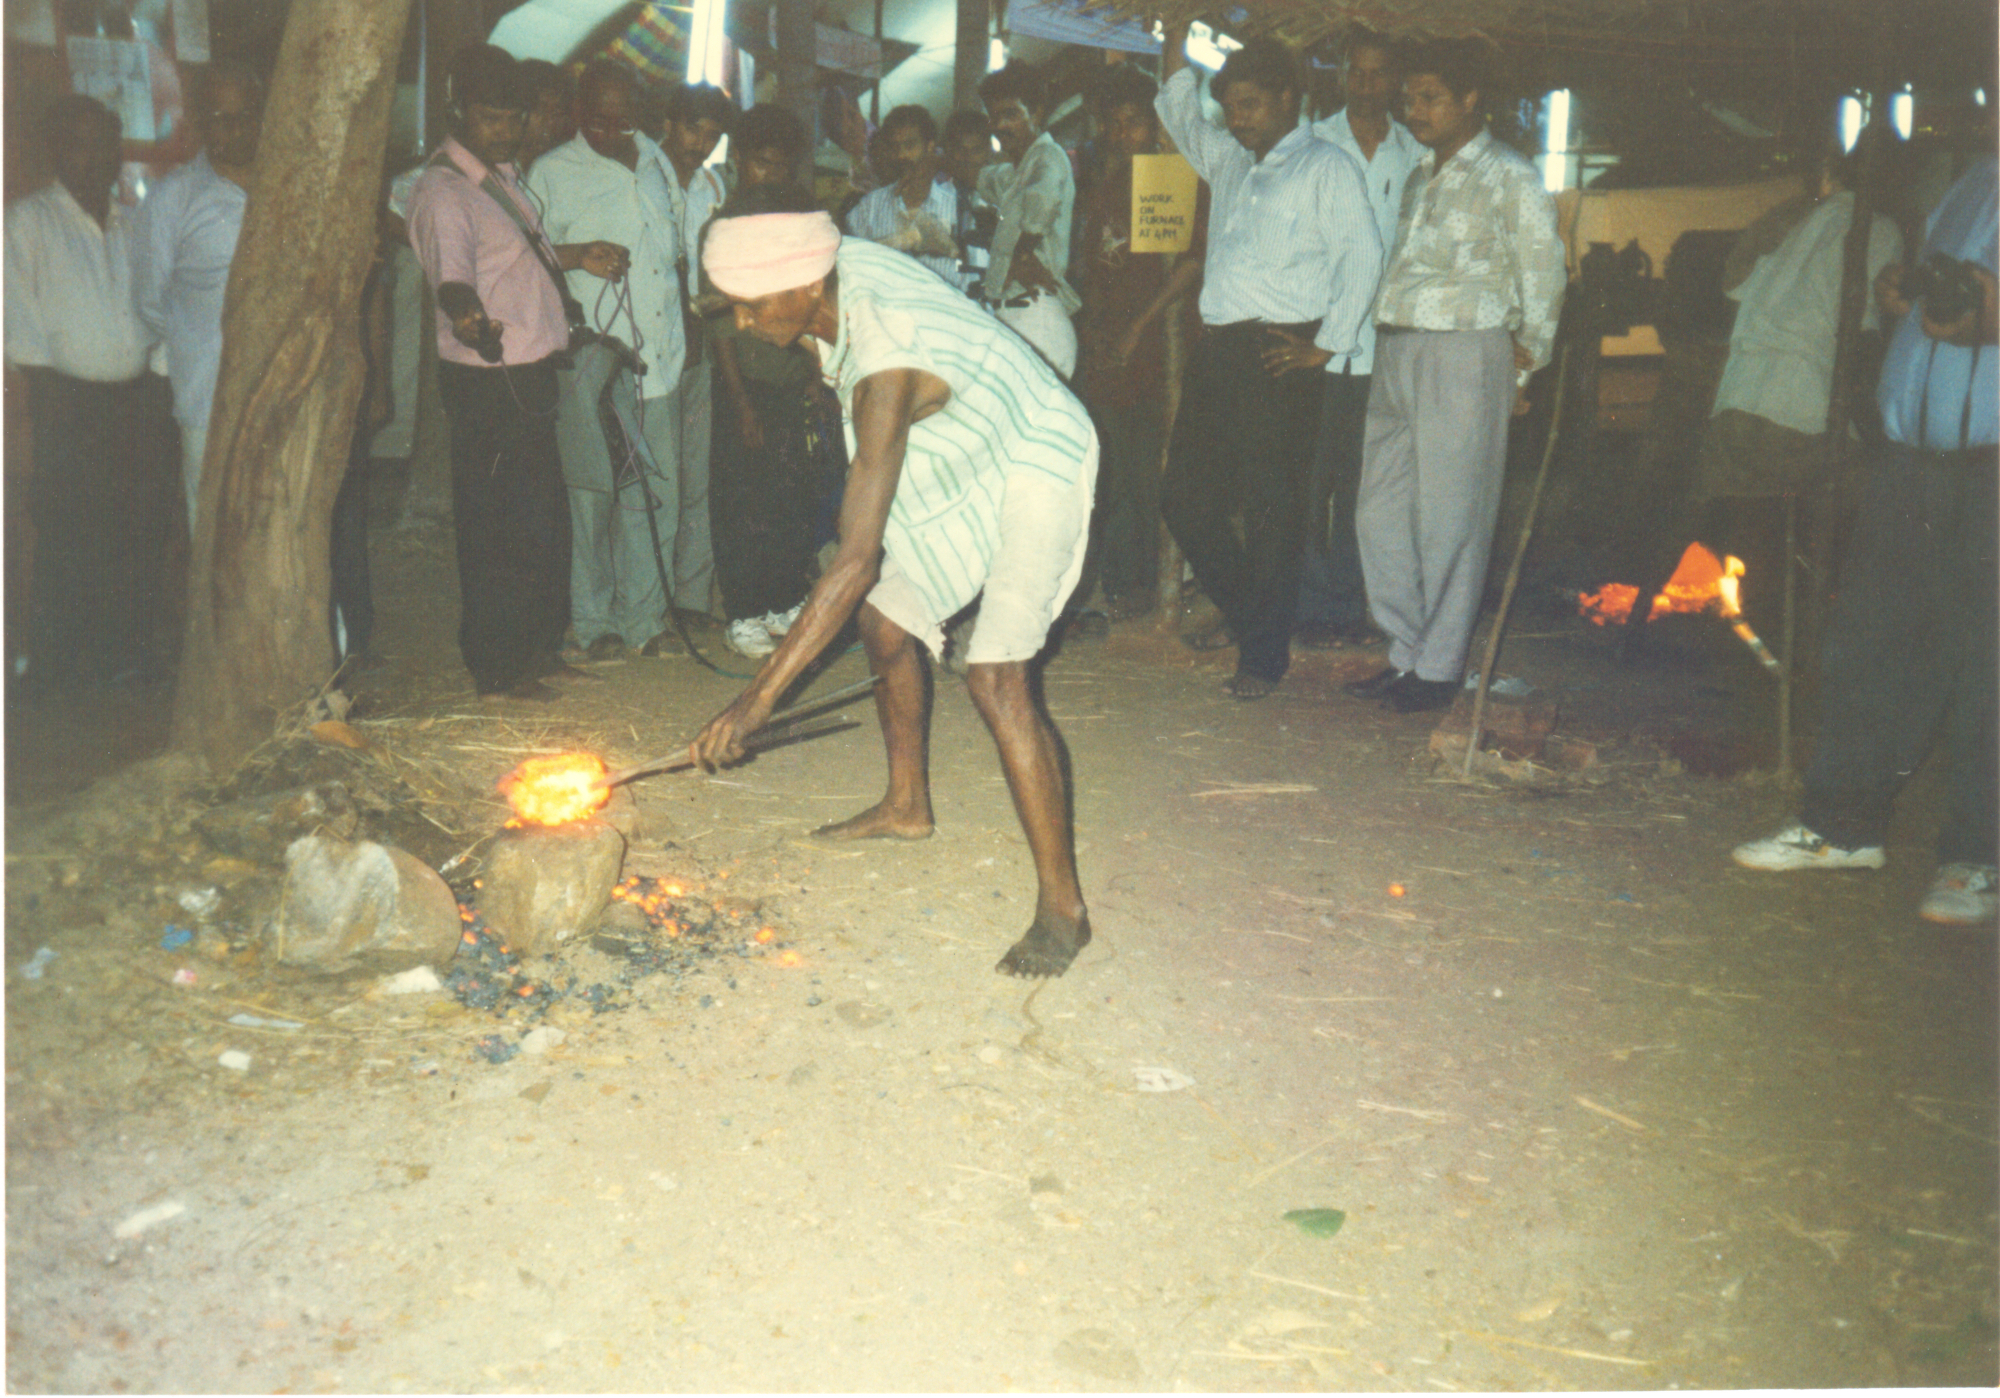
\includegraphics[scale=0.58]{images/chapter-7/fig045D.jpg}
\caption{Agaria smelters at work, Balaghat}\label{chapter-7-fig45D}
\end{figure}

\noindent \textbf{\large 4.~Furnaces}

Small sized furnaces are in vogue among most of the traditional societies, including in the area we have studied. For preparing the furnaces, locally available clay is used. Straw or rice-husk is mixed with the clay and soaked for a long time and kneaded thoroughly. The smelters do not use any scales for measurement but use their fingers ({\it anguls}) instead. For preparing the furnace, first of all a pit of about 8 inches or 14 {\it anguls} deep and of the same diameter is dug in the ground. A channel of the same width is dug joining this pit at its right angles from the main opening of the furnace under preparation. Three sticks are stuck around the base-pit providing the basic foundation structure for erecting the furnace wall, which is about 5-6 inches or 14-15 cm. thick (Fig.~(\ref{chapter-7-fig47C} \& \ref{chapter-7-fig50}). The outer diameter of the furnace is 20 to 22 inches or roughly 50 60 cm. at the base and tapers to about 16-18 inches 45-50 cm. towards the top. The mouth of the furnace at the top is six inches at the opening and becomes broader towards the base. It is this tapering hole, which holds the main charge. To slide the charge into this hole an ovalish or rectangular platform or saucer like structure of one and a half ft. diameter around the mouth of the furnace and this is slightly pointed and conical on one side, aptly called {\it argha} is made (Fig.~\ref{chapter-7-fig44D}). Another opening is made at the surface level. It is 8-10 inches wide and about 10 inches high. It is used both for inserting the bellows through a tuyere and for removing the bloom at the conclusion of the work. During the operation, this opening is sealed with a mixture of ash and mud. After the furnace structure is ready, it is allowed to dry. At this stage a paste of some special smooth, yellowish clay is applied on the inner side of the structure. The workers believe that this paste affects the smelting process as well as the quality and quantity of the end product. This appears to have properties, of a fluxing agent. Though, the clay of this paste has yet to be analysed for its properties.

Bellows are made of cow or buffalo hide, mounted on a special wood hollow of about 14" (35cm) circumference are used (Fig.~\ref{chapter-7-fig46B}). Twin bellows attached through a clay tuyere to bamboo sticks are used. The bellows are operated alternately with foot with the support of sticks with a frequency of 120-strokes/per minute giving a flow rate of 100 l pm. As the activity gains momentum, the rate of strokes per minute increases. It rises up to 150-160 towards the peak hours. It slows down towards the end of the smelting process.

The process begins with some religious rights and offerings to their deity praying for successful conclusion of the operation. The furnace is charged with alternate layers of charcoal and ore. After the furnace has been ignited and the bellows start blowing air with full blast, additional charge of ore, alternated by charcoal which is piled on the top of the platform or {\it argha} or the platform to be later pushed into the furnace. This process probably pre-heats and removes moisture from the charge. Nearly 15-20 Kg of ore and 30-40 Kg of charcoal is used up in one operation lasting for about 3-4 hours. As pointed out earlier, where a better quality of ore is available, like at Pratappur, the amount of ore and coal that is consumed is comparatively lesser i.e., 15-16 Kg of ore and 25-30 Kg of charcoal. At intervals, the slag is tapped with a thin stick through the channel at the side of the furnace. The molten slag runs out of this in a red-hot condition (Fig.~\ref{chapter-7-fig45C} and Fig.~\ref{chapter-7-fig51}, the latter is from Pipra, Sidhi). The opening of this channel is sealed in the same way as the aperture for bellows. A hole may be made into this loosely sealed opening by simply poking a thin rod raking the charge a bit, so that the liquid slag flows out of the furnace. The bellows are operated at a faster and quicker pace at the peak, gradually slowing the pace towards the end. The master artisan makes an assessment at this stage whether the iron is ready. The bloom is then removed with a pair of tongs through the opening by removing the bellows, tuyeres and the temporary seal of loose clay and ash etc. Generally, approximately 3-4 Kg of iron is produced depending on the quality of the ore and the success of the working. Efforts of revival of tribal smelting have been made in several other parts of the country. Mention may be made of Asur-Birjia of Netarhat plateau, Jashpur Agraria, Ghatgaon Agraria and those living in parts of Orissa. Some of these efforts that proved successful are briefly described here. It may be noted that although they look more or less identical, there are some fine differences in the basic method of working of these groups. This may well be minor adjustment made to suit the local raw material specifications that must have evolved over time.

\begin{figure}[H]
\renewcommand{\thefigure}{46A}
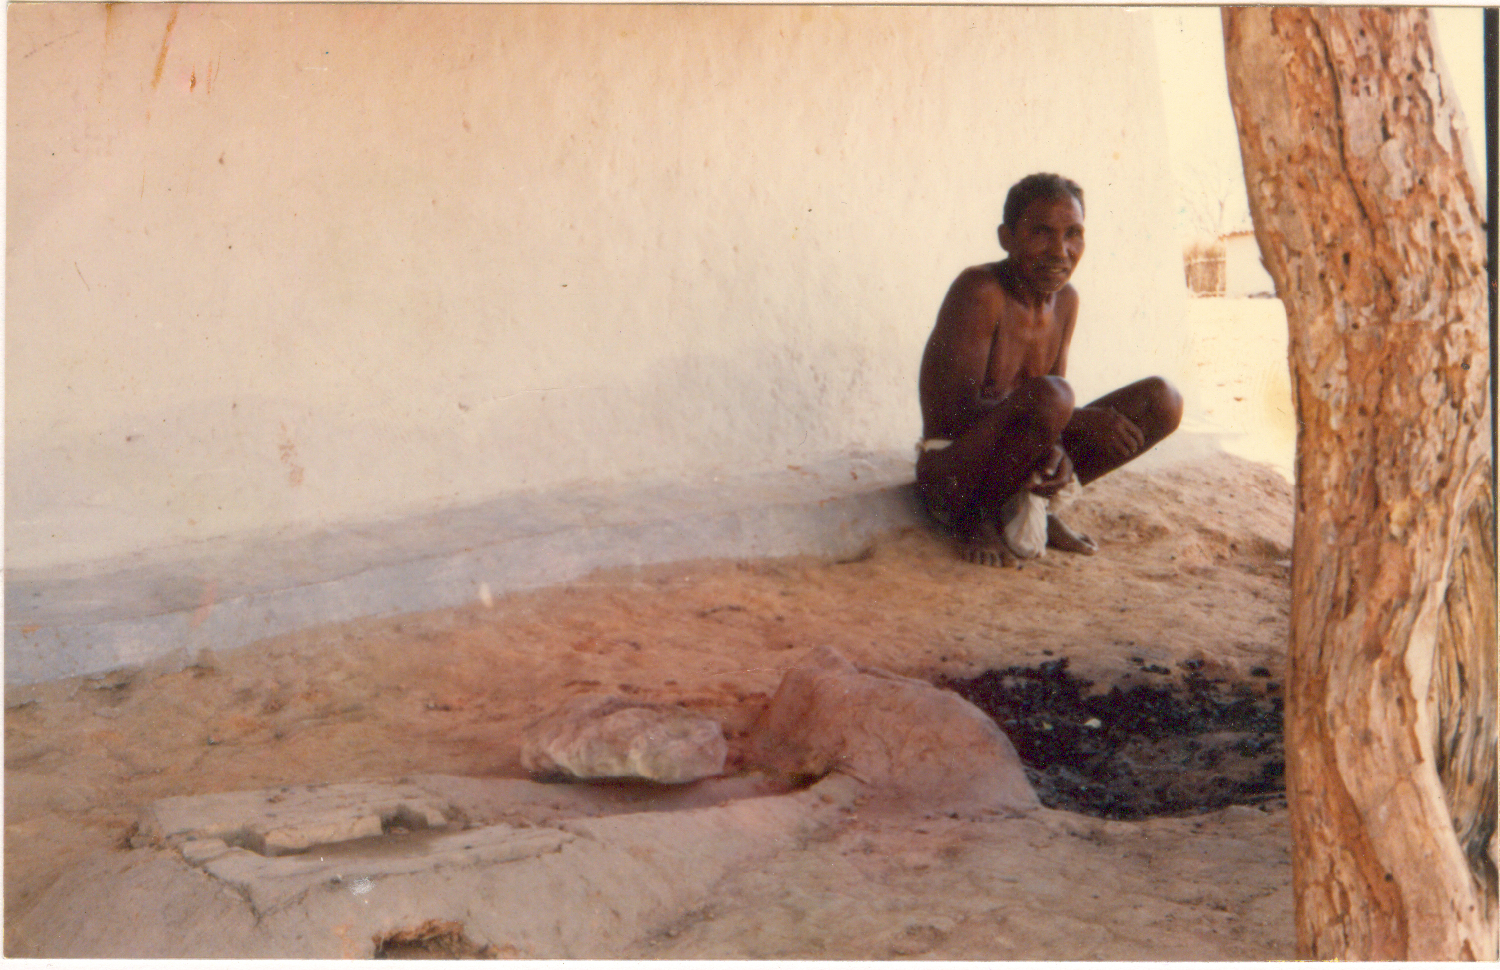
\includegraphics[scale=0.78]{images/chapter-7/fig046A.jpg}
\caption{Iron forge at Wadruffnagar}\label{chapter-7-fig46A}
\end{figure}
\begin{figure}[H]
\renewcommand{\thefigure}{46B}
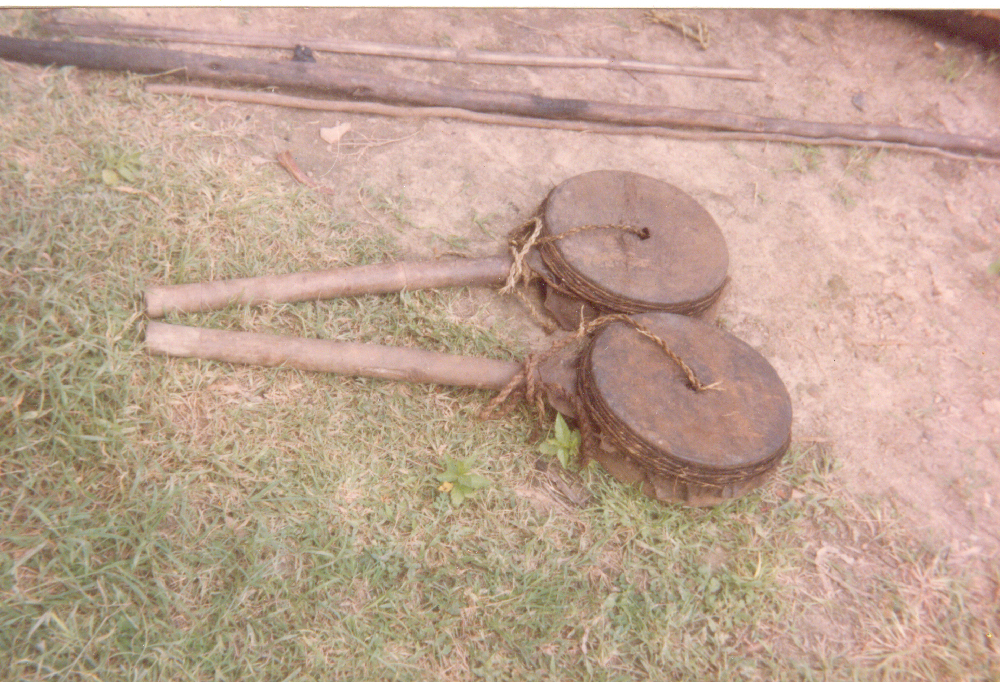
\includegraphics[scale=1.15]{images/chapter-7/fig046B.jpg}
\caption{Bellows Wadruffnagar}\label{chapter-7-fig46B}
\end{figure}

\newpage

\begin{figure}[H]
\renewcommand{\thefigure}{46C}
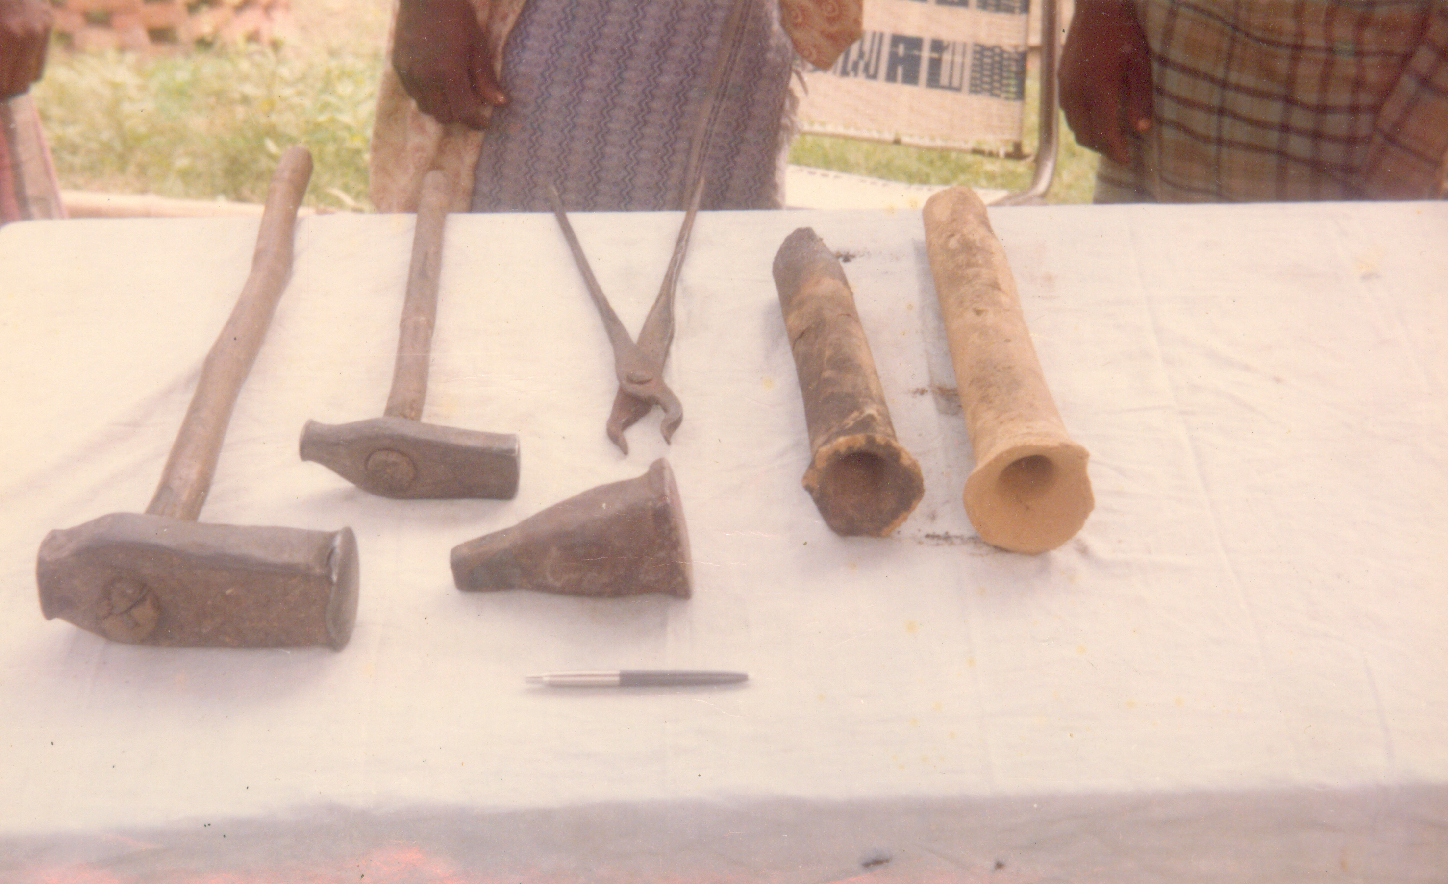
\includegraphics[scale=0.8]{images/chapter-7/fig046C.jpg}
\caption{Tools for iron working at Wadruffnagar}\label{chapter-7-fig46C}
\end{figure}
\begin{figure}[H]
\renewcommand{\thefigure}{47A}
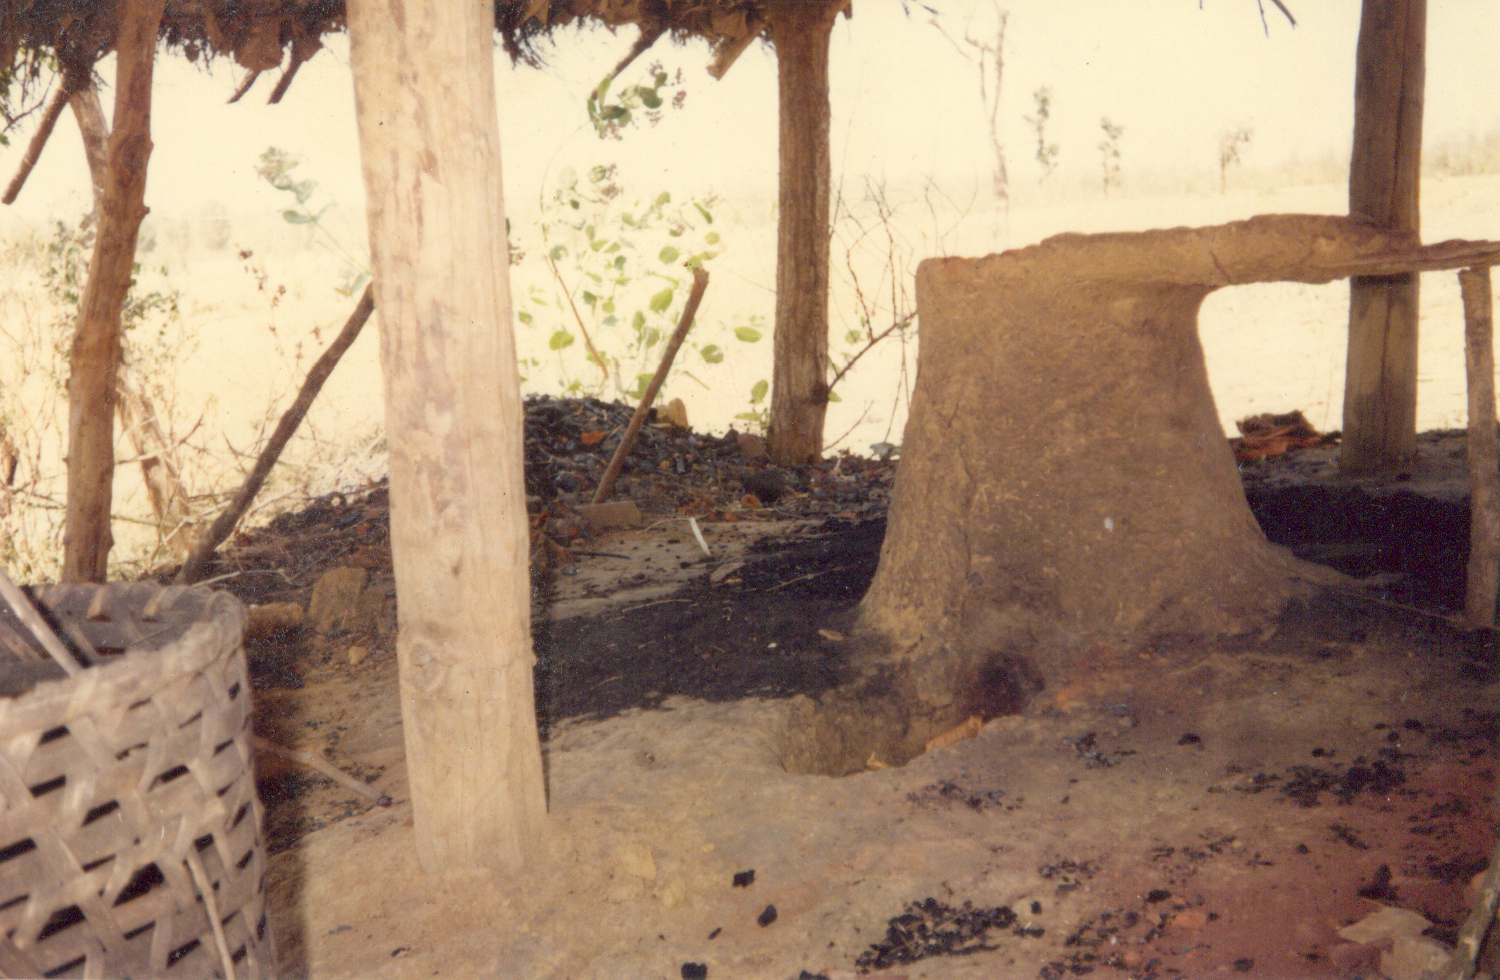
\includegraphics[scale=1.55]{images/chapter-7/fig047A.jpg}
\caption{Furnace in use at Kathua, Pratappur}\label{chapter-7-fig47A}
\end{figure}

\newpage

\begin{figure}[H]
\renewcommand{\thefigure}{47B}
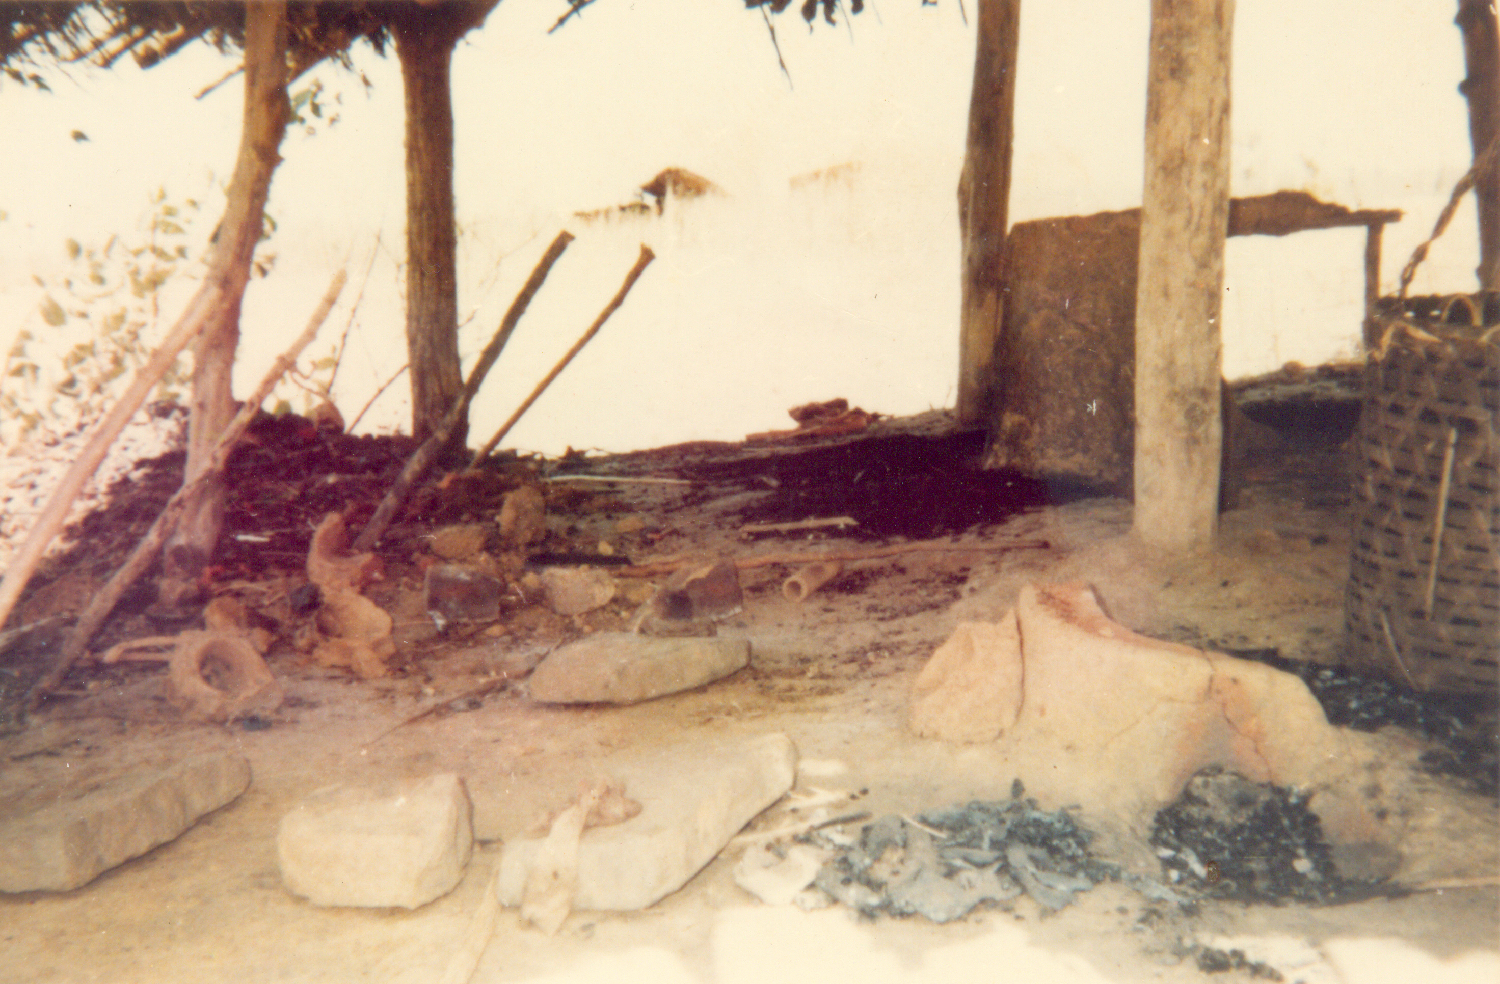
\includegraphics[scale=1.5]{images/chapter-7/fig047B.jpg}
\caption{Furnace in use at Kathua, Pratappur}\label{chapter-7-fig47B}
\end{figure}
\begin{figure}[H]
\renewcommand{\thefigure}{47C}
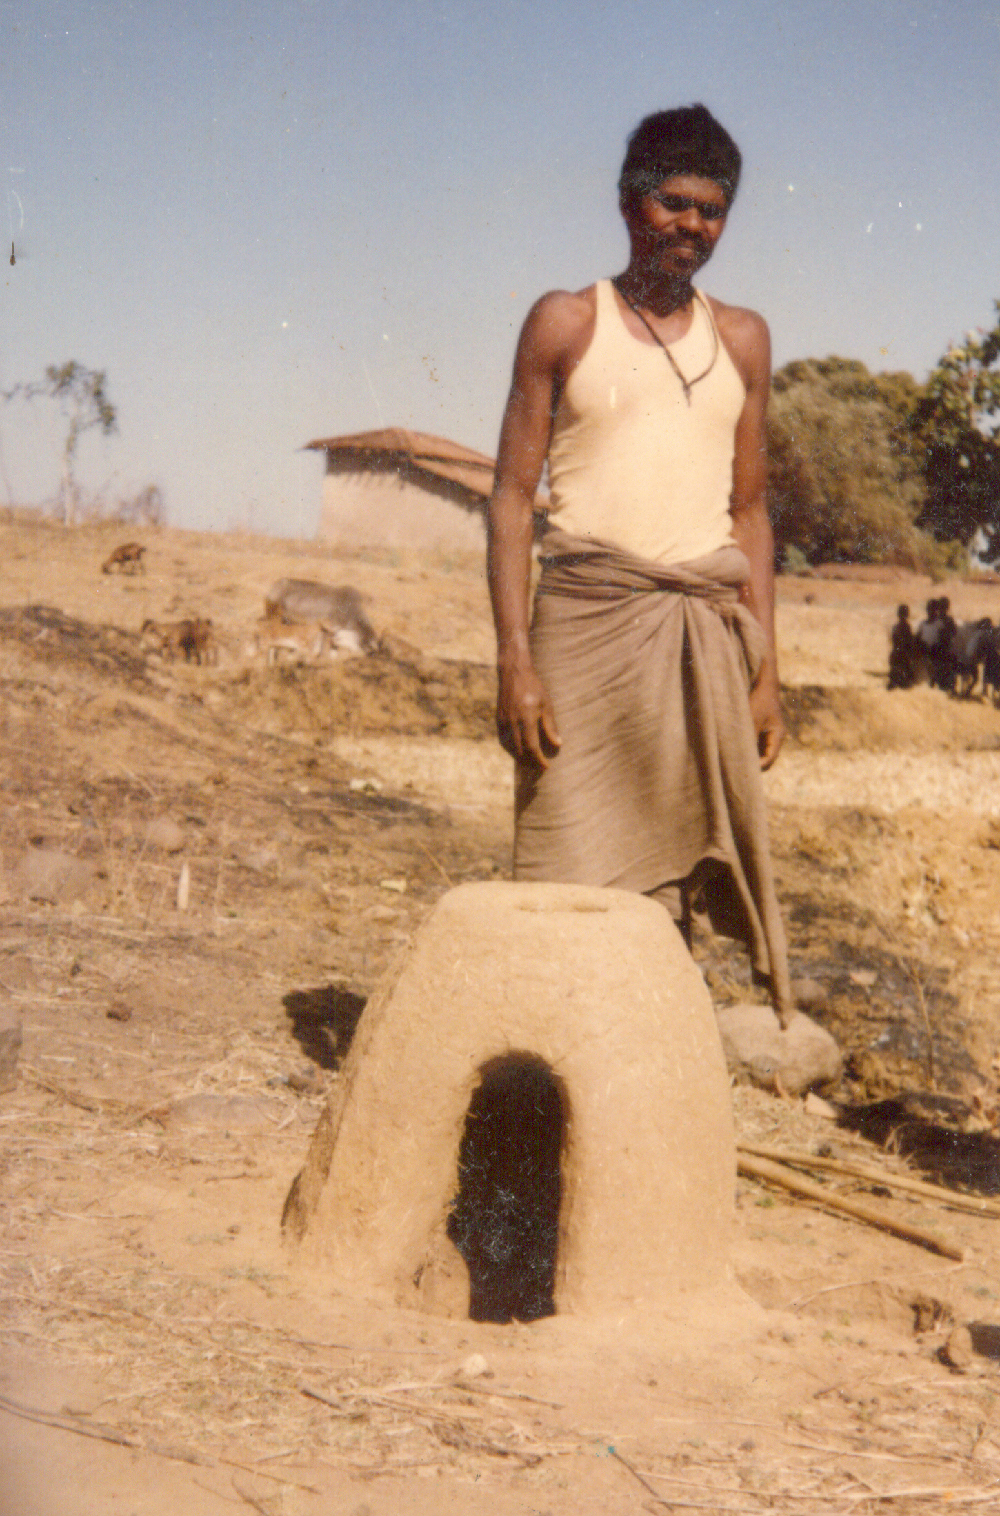
\includegraphics[scale=1.2]{images/chapter-7/fig047C.jpg}
\caption{Furnace at Kathua, Pratappur}\label{chapter-7-fig47C}
\end{figure}

\newpage

\begin{figure}[H]
\setcounter{figure}{47}
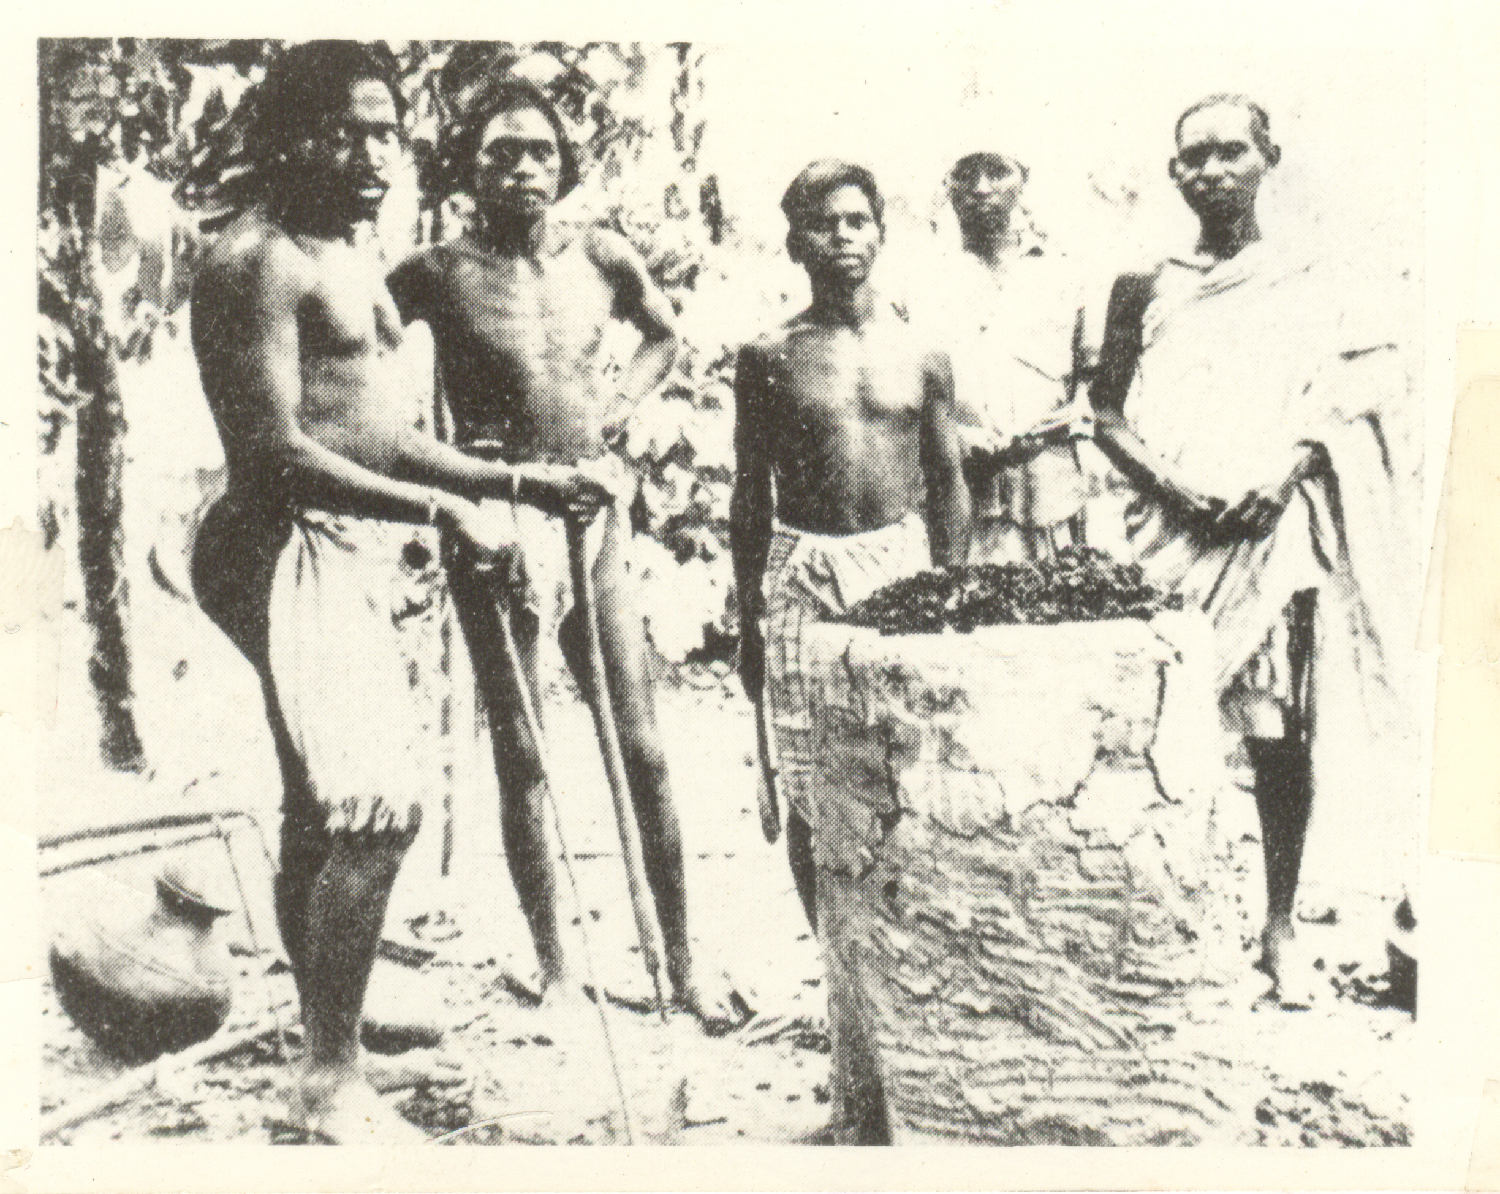
\includegraphics[scale=1.5]{images/chapter-7/fig048.jpg}
\caption{Agaria iron Workers with their furnace, Ranchi}\label{chapter-7-fig48}
\end{figure}
\begin{figure}[H]
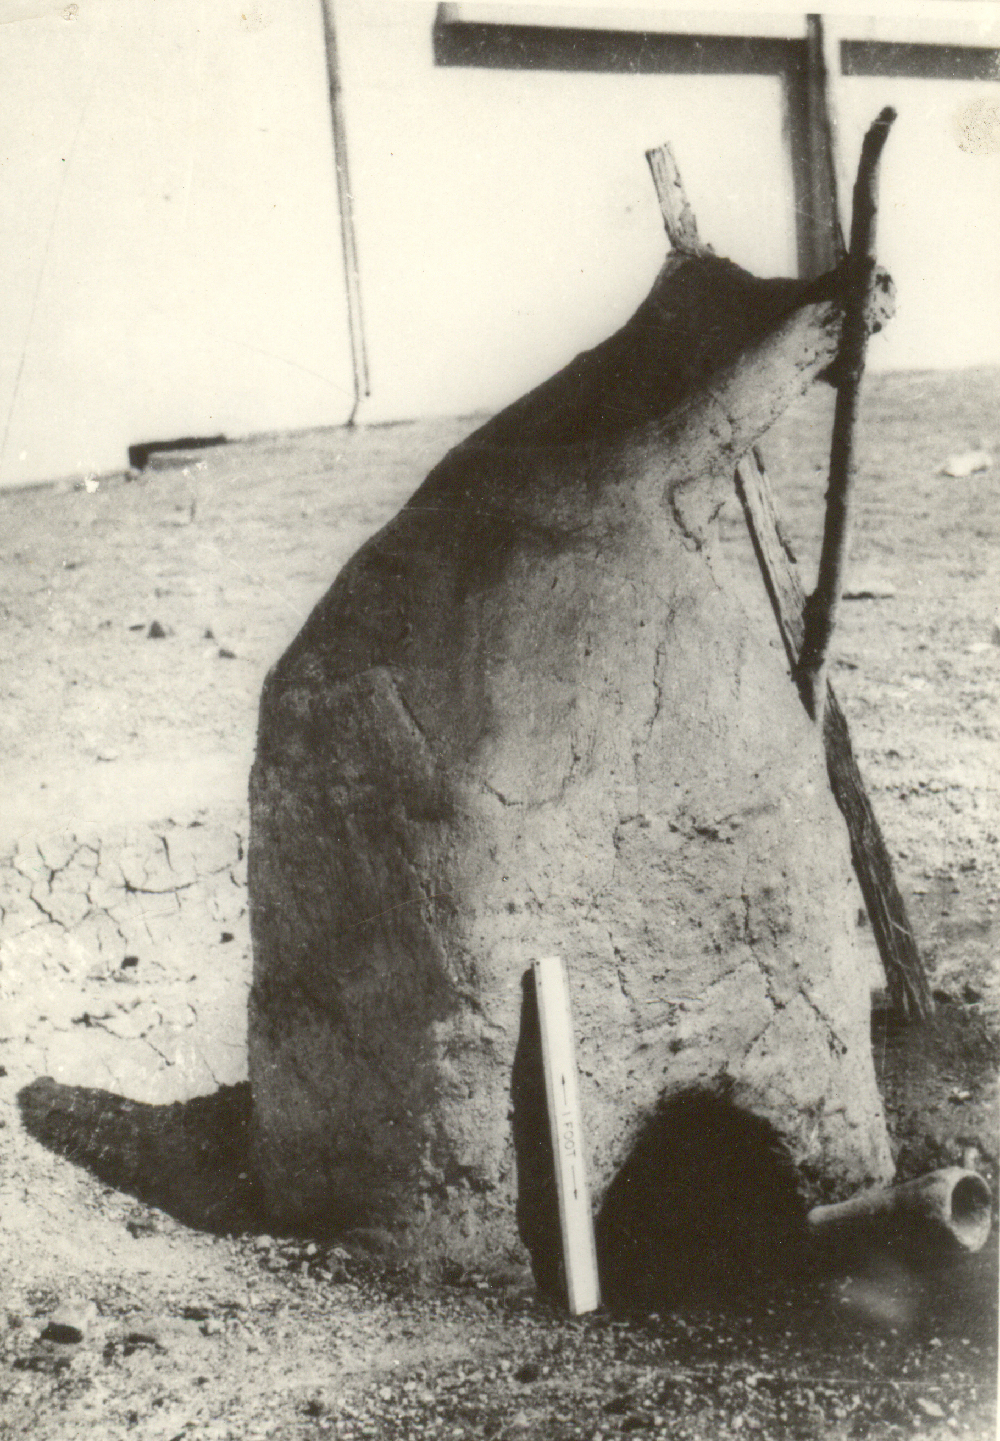
\includegraphics[scale=1.1]{images/chapter-7/fig049.jpg}
\caption{Pre-industrial Furnace, Nagpur}\label{chapter-7-fig49}
\end{figure}

\newpage

\begin{figure}[H]
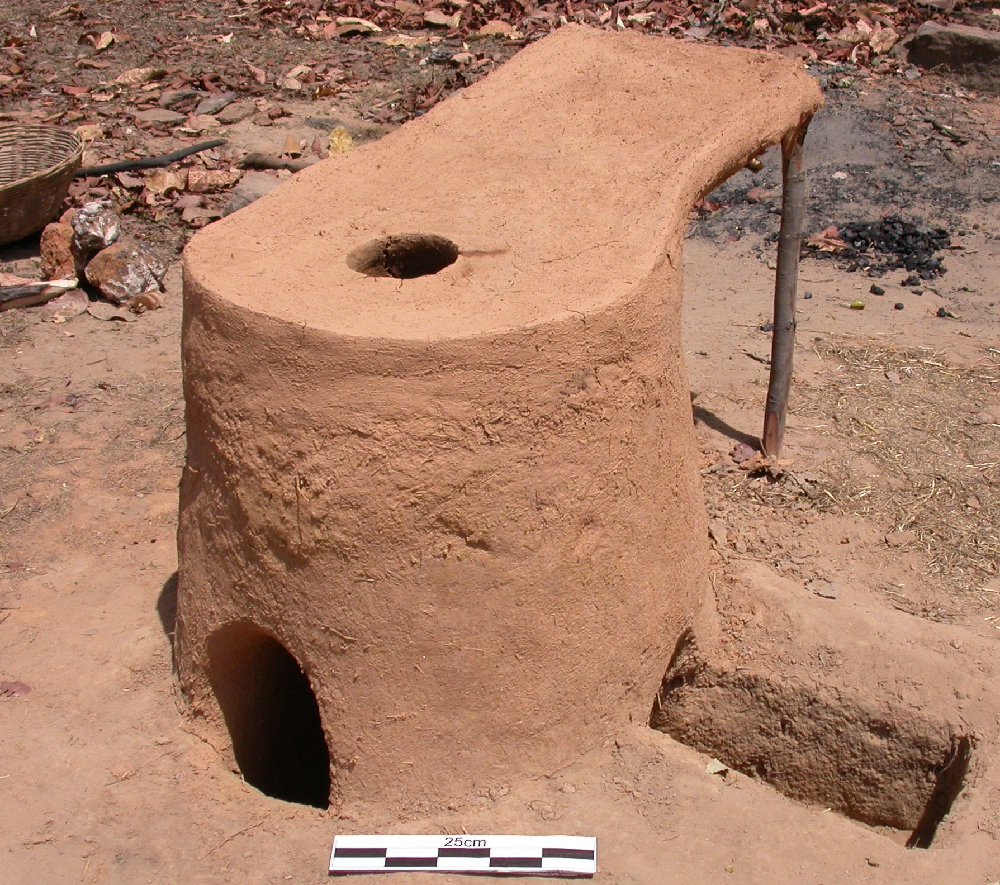
\includegraphics[scale=1.1]{images/chapter-7/fig050.jpg}
\caption{Furance ready for smelting, Pipra, Sidhi}\label{chapter-7-fig50}
\end{figure}
\begin{figure}[H]
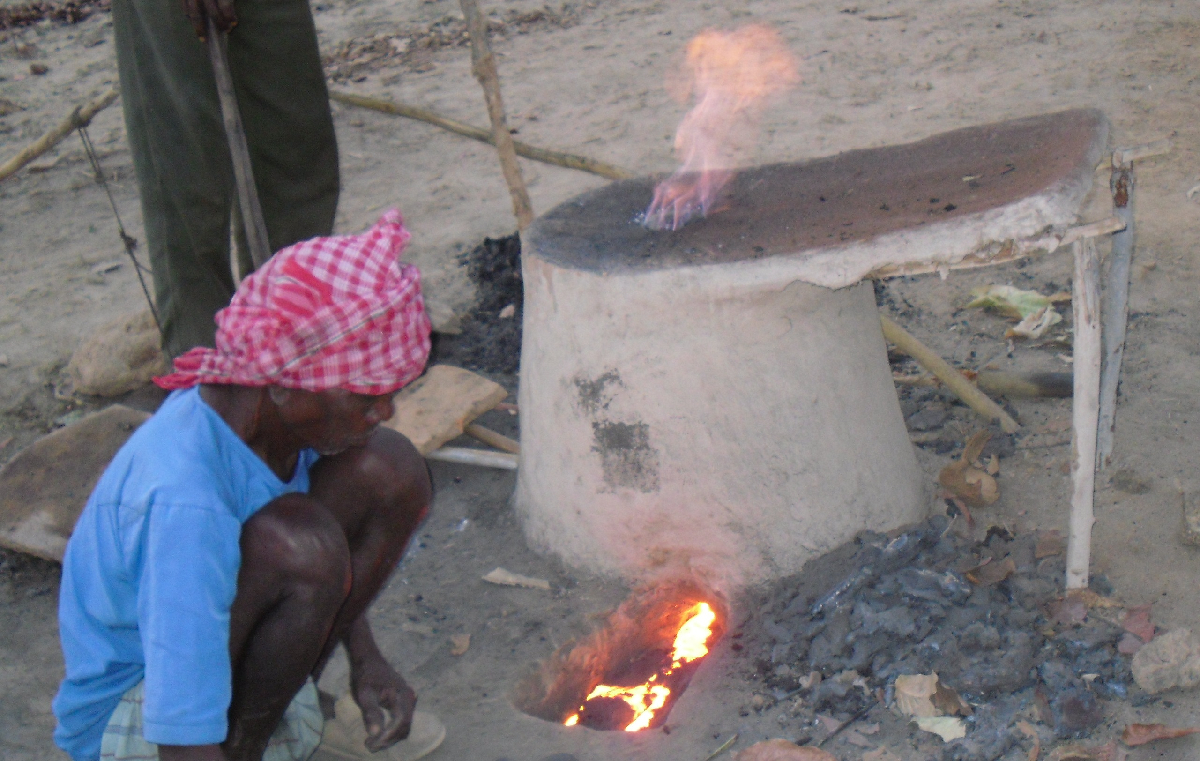
\includegraphics[scale=1.6]{images/chapter-7/fig051.jpg}
\caption{Furnace in operation, molten slag being tapped out of the channel. Note the stone slab used to weigh down the bamboo-pipe attached to bellows-Copy}\label{chapter-7-fig51}
\end{figure}
\vspace{-.4cm}

\subsection*{Iron making in Netarhat Plateau – Jharkhand}\label{chapter7-subsection-7.1b}

\vspace{-.3cm}

The traditional smetters of Chhotanagpur Division of Jharkhand have been found to be practising an earlier iron making technique. Evidence of the same was located on and near Netarhat Plateau. A few old artisans were located who had practised the art till almost 50 years earlier. Vikash Bharati, a regional centre for appropriate rural technology, has located the "Asur Birjia" community in Garha Harup Village on Netarhat Plateau (near Bishunpur on Lohardaga-Netarhat Road) who practised an ancient process of iron making to make implements for their use. The Research and Development Centre of Iron and Steel (RDCIS), SAIL, Ranchi made an attempt to study and characterize the process.

A vertical shaft type furnace is used there. Lumps of iron ore and charcoal from sal wood are the only raw materials. Feet operated bellows are used. The furnaces produce sintered lumpy sponge iron (some liquid slag which is generated during operation is tapped beforehand). Sintered lumpy sponge iron is repeatedly heated in a separate furnace and beaten to give final shape to finish the implements. 
\medskip

The Scientists at Research and Development Centre of Iron and Steel (RDCIS), at SAIL, Ranchi initiated investigations by temperature measurement and analysed the iron ore, charcoal, tuyere, refractory clays, sponge and metal. These samples have been subjected to variety of examinations, such as chemical analysis, optical microscope and scanning electron microscope examinations as well as other physical tests.

Studies indicate that this process operates at a temperature midway between the direct reduction and liquid iron making process temperature. The temperature attained in the tuyere region is as high as $1500^\circ$ C. The total iron content of sintered sponge iron is only 55\%. The final product obtained after reheating and beating contains around 96\% iron, the balance being $FeO$ and gangue. 

The natives of Ghatgaon near Jashpur of Bastar region practice a process, which again uses a shaft type furnace, made of local mud. It is heated with charcoal (of {\it sal} wood) and then iron ore fines (washed iron ore fines are collected from the bed of an adjacent river) are sprinkled into the furnace from the top along with some more charcoal. The end product is a sintered sponge iron and some liquid slag. The process may be compared with the modern fluidized bed process where gases are used to serve the dual purpose of fluidizing media and the reducing agent. In a general way, the Bishunpur and the Jashpur processes appear similar.

\noindent \textbf{\large 5.  Forging}

In an open hearth, which is simply a shallow pit full of red hot burning coal, also sometimes worked with bellows, the bloom is heated up to $700^\circ-800^\circ$C and hammered with a heavy sledgehammer (Fig.~\ref{chapter-7-fig45D} and \ref{chapter-7-fig46C}) This process is repeated several times. The impurities trapped in the form of sintered slag are pushed out of the bloom attributing in compactness and homogeneity as well as some hardness on the surface because of a prolonged direct contact with charcoal i.e., carbon. Iron thus produced by these traditional smelters is preferred to the factory-produced iron by local people because of its high quality, durability, ductility and capacity to provide better cutting edges.	

A close observation of metallurgical processes brings out special features of pre-industrial metallurgy which may be enumerated below:

\begin{enumerate}[a)]
\item The size of the furnace is very small, barring a few exceptions. The height of furnace varies between 0.6 and 1.2 m and diameter at the bottom about 0.25-0.5m.
\item Charcoal is the fuel used. The Madhya Pradesh-Chhatisgarh tribes use {\it sal} or {\it sarai} wood for charcoal. This is a purer material having lower sulphur and phosphorus. The metal thus produced is naturally low in sulphur. Phosphorus is the only element, which remains in the metal produced with ores, from its natural composition. (Ballal et. al. op.cit.)  	
\item Generally, no basic ($CaO$) flux is used, even when lime is easily available which removes sulphur from the end product. Instead, calculations by Prakash have shown the use of extra $SiO_2$ (sand) as acidic flux in the charge.
\item The smelting process is usually described as wasteful and low yielding. About 4-5 Kg of iron may be produced after utilising about 15-20 Kg of ore.
\item The high percentage of charcoal used in traditional working has several advantages. When the charcoal proportion is high (Tylecote et al. 1971) the metal contains more carbon. We have stated earlier that the Chhattisgarh smelters use about 30-40 Kg of charcoal for 15-20 Kg ore, i.e., more than double the amount. Hughes, reporting on Central Province iron smelting (1873) states that for production of 1 Kg of bloom 3.6 Kg of ore and 4.97 Kg of charcoal was consumed. The bloom was then refined twice, which caused it lose substantial weight. The charcoal was produced in circular kilns or alternatively by piling the logs in open fire, (Fig.~\ref{chapter-7-fig56}-\ref{chapter-7-fig57}). The latter, it may be said is a more wasteful process.
\item The temperature in the furnace is not uniform. It is low-around $600^\circ$C in the upper portion, going up to $1300^\circ$ C- $1400^\circ$ C or some times nearly a high as $1500^\circ$ C near the tuyere zone. A close study of the whole production process and temperature mechanism has led metallurgists to believe that ``… the traditional smelter is constrained by the low temperature in the furnace and the process is finely tuned to his requirements, any rise in the slag melting temperature can ruin the product... " (Ballal et. al.) 
\item The tribal smelters are almost religiously careful about the specific type of wood which they use for making charcoal to use as fuel, clay that they use, time and spot for smelting (supposedly, humidity in outside temperature affects their working) and about the type of ores that they use. They do not wish to experiment with their working in any way. Magnatitic sand from rivers has been used by several such groups because of its purity and other advantages.
\item It has already been pointed out that the metal produced traditionally is of higher quality. It is well known, concludes the report of I. I. T. Bombay Metallurgical Engineers, ``that small blast furnaces operated with charcoal give superior metal product. "
\item The smelters were capable of producing a variety of iron like the famous wootz steel of south India, of course through a different technique. Apparently, a similar white iron or {\it Charka Loha} is produced in Sarguja district of Madhya Pradesh using magnetic sand. The Parsa group of the {\it Mahuli Agarias} are adept in this art and the product is used for making weapons. It is of a much superior quality and is much more expensive. The metallurgical skill however, is exclusively restricted to only a small tribal group of artisans who have perfected it over the period.
\end{enumerate}

\vspace{-.5cm}

\subsection*{Discussion}\label{chapter7-subsection-7.1c}

\vspace{-.2cm}

We may now look at the nature of iron working, its suitability, viability etc. in the present day context. The issue, which deserves a serious consideration here, is whether it is eco-friendly.

\begin{enumerate}[1)]
\item First, a closer look at the consumption of ore and charcoal, the two indispensable raw materials of the iron smelting is called for. Do we see a thoughtless or callous exploitation by these communities? Many early studies have attributed wastefulness to traditional iron smelting. Quite a sizeable percentage of iron remains in the matrix of slag. 15-20 kg. of ore yields only 4-5 kg. of bloom which loses further weight in the forging  and refining process. This calculation, however, ignores the fact that these ethnic societies are tapping those ores which are many a times rated low grade and not even considered worth smelting. Significantly, they also locate those small pockets of ore deposits that have not been even recorded in geological texts listing only economically viable deposits. In our considered opinion {\it it is a maximisation of resource utilisation}. We have already described the gentle way of ore-picking by these groups. The tools and implements used by them are of very simple type (Fig.~\ref{chapter-7-fig46C}).

As pointed above it may be emphasised in this context that, they also make use of magnetitic sand from rivers. Thus they utilise a waste material that would otherwise be washed away and wasted. Can there be a better example of human enterprise in the modem world? Thus by no standards this working may be called extravagant, so far as the utilisation of ore is concerned.
\item The indigenous iron working used charcoal for energy. Thus the biggest irritant in the modern times of ecological consciousness is use (or misuse!) of wood for charcoal making a major justification for imposing a ban on this household industry. 

The Agarias, reported Verrier Elvin (1942, p.121.) lived near the forests, (see Agaria belt, Fig.~\ref{chapter-7-fig42}) ``where there are sarai trees, there you will find Agaria”. {\it Sal} or {\it Sarai} is the tree favored for charcoal by Chhattisgarh and Sarguja Agarias too\endnote{Experiments carried out by Prof Bhanu Prakash and the author with Waddraffnagar Agrarias have shown that even poor grade charcoal could be used in these furnaces but for this the smelters have to be trained and prepared mentally to change the air blowing rate.}. Though they also use tamerind {\it Bija, Mahua, Babool} and {\it Bamboo} etc. for various proposes in the course of smelting. 
\end{enumerate}

What has been overlooked in our calculations however is that there are taboos, sanctions, religio-social prohibitions on indiscriminate cutting of trees. Mostly charcoal is made from with dead trees lying around in the forest. The trees as discussed earlier, in the jungle are thought to be abode of deities or spirits of ancestors who look after taking care of their welfare. If a fire breaks out in the forest, around Dhenkanal in Orissa every family has to participate in putting out the fire or else they have to face social sanction inform Walter Fermandes, Geeta Menon and Philip Vegas (1988, p.168) on the basis of their study in the specific context of Orissa. The study further reiterates the economic measures taken by such groups in the use of forest resources. For instance, the Agaria families of Chattisgarh and Chhotanagpur which visit the jungle for coal making collect, pile and burn the wood for charcoal. They also collect and bring back {\it Sal} leaves to use as plates for meals. It is noteworthy that even the number of leaves a family can pluck is rationed. 

It is noteworthy that even leaves cannot be plucked indiscriminately or carelessly, what to speak of trees? They have a sanctity, honour and respect for the trees in general. It is amply demonstrated during {\it Karma} Festivity. It is this kind of fully internalized respect for nature, especially trees which helped the survival of both the traditional industries as well as forests. Maximum threat to the forest has been posed by indiscriminate scavenging of trees in recent years when the forest dwellers were dispossessed and displaced from their age-old habitat. Both the jungle and the man have suffered due to this so-called modernization or acculturation process.

\vspace{-.3cm}

\subsection*{Economic Viability}\label{chapter7-subsection-7.1d}

\vspace{-.2cm}

We have considered the status of the resource management techniques of the traditional workers of the indigenous iron industry. Let us now discuss in the present situation its economic viability. If we compare the small-scale industries with the mechanised mass productions, this is incommensurable. The native techno-systems are prone to wilt and wither away in the face of the aggressive onslaught of modern technology. Our surveys reveal that by and large smelting is an abandoned practice and a story of the past (Fig.~\ref{chapter-7-fig52}-\ref{chapter-7-fig53}). Could there be a comparison between the hand spinning and weaving on looms and cloth mills?

Yet the planners have protected and subsidized, facilitated weavers in post-independence era. There could be many such examples in need of similar sympathetic consideration. A proposal of this nature was given in the report and suggested by the first planning commission of India immediately after independence.  

Some calculations may, however be made here in support of our contention. The furnaces in our area of investigation and also in most of the other areas are small, yielding only a small amount of iron per smelting charge. On the basis of Geological Survey of India reports of the pre-independent era, our calculation (Tripathi and Tripathi, 1994) are that, per kg of refined iron needs 7.92 to 9 kg. iron ore 14.62 - 16.71 kg. charcoal made out of 50-60 kg of wood. The smelting operation lasts for 4 to 6 hours, depending on the type of raw material being used. The consumption of charcoal, thus appears heavy enough justifying ban on iron production by the traditional workers. But the question is whether it is really uneconomical and hazardous to ecological balance? The traditional iron working must be viewed in the totality of its context. We have seen earlier that ­ -

\begin{enumerate}[1)]
\item The ethnic smelters use 
\begin{enumerate}[(a)]
\item low grade ores, 
\item if high grade ores like hematite and magnetite are used, nodules are hand - picked or at the most chisels and mattocks are used for very shallow digging without defacing the surface by deep digging; 
\item magnetitic river sand is used at several places; 
\item minor pockets of ore deposits are utilised, generally. 
\end{enumerate}
Thus ore-wise these groups are almost parsimonious, many a times utilizing the so called rejected materials!
\item Charcoal is the most difficult part in today's context. But we need to bear in mind that it is a renewable resource. This can be resolved by giving a 20-25hactare land between 10-12 villages for survival and revival of an ancient industry. This will ensure 
\begin{enumerate}[(a)]
\item a decent living, 
\item job opportunity, stability and 
\item the revival of a high quality product of immense techno-cultural value to India. This iron because of its superiority are preferred by the users in nearby villages even today though it is slightly more expensive than the factory made iron objects, 
\item most of all, the preservation of cultural ecology in an otherwise endangered social set up involving a fairly large population. 
\item In the longer run this may also help in revival of regeneration of forest products and (which are now vanishing fast) of the jungles to be used by these communities. 
\item Thus it will ensure a more stable eco-system or ecological balance - both natural and cultural.
\end{enumerate}
\item It is possible to maintain equilibrium between natural resources, expenditure and ecological regeneration if efforts are made. An estimate was prepared for regeneration of forest resource towards revival of the art-craft (or technology?) of iron production while it also provides job opportunities to a large populace which is deprived of its traditional profession. A group of metallurgical Engineers of IIT Bombay worked on this problem and arrived at the following conclusion, which is self-explanatory.
\end{enumerate}

Cutting down virgin forests for the charcoal is economically and ecologically disastrous indeed. But it is possible to grow trees on a sustainable basis on wastelands "... it becomes almost a zero pollution industry. The cost of carbon dioxide generation during the burning of charcoal has already been paid while growing the trees". (page 96 of report). The report further concludes, 

{\fontsize{9}{11}\selectfont\begin{longtable}{|l|l|}
\captionsetup{font=small}
\caption{Preliminary Details (SAIL)}\label{table 8.3}\\
\hline
Charge weight & 20 kg.\\
\hline
Iron ore & 20 kg.\\
\hline
Charcoal & 0.3 kg.\\
\hline
Limestone & \\
\hline
Total time taken & \\
\hline
for tapping & 04 hours\\
\hline
for forging & 04 hours\\
\hline
Wrought iron product  & 06 kg\\
\hline
Finished weight & 04 kg\\
\hline
Number of implements made & 20\\
\hline
Number of persons engaged& Two\\
\hline
Cost & Rs.\\
\hline
Cost of mineral inputs & 4.00\\
\hline
Cost of charcoal & 30.00\\
\hline
Incidentals & 6.00\\
\hline
\textbf{Total} & \textbf{40.00}\\
\hline
Value of output & \\
\hline
reckoned at current price & 100.00\\
\hline
Available surplus & 60.00\\
\hline
Earning per head/day & 30.00\\
\hline
\end{longtable}}

\vspace{-.2cm}


"If a 50 year cycle of plantation and harvesting is adopted, the average yield works out to $4m^3$ of dry wood per hectare per year. At an average density of $750/m^3$, the yield is 3 tonnes of dry wood per hectare, per year. To support one furnace, therefore, 20-25 hectares of land under {\it sal} plantation in required. A furnace operating without break for extended periods of time and working for about 300 days in a year, needs about 20-25 hectare of land for supply of wood on a sustained basis and can cater to the needs of 10-12 villages". (Ballal {\it et.al.}). Similar suggestion was offered by Leuva as pointed earlier.

As early as 1882, the European engineers had also tried to work out the possibility of iron production with charcoal in certain parts of India. Special mention may be made of Schwartz. He had studied the ores of Lohra and Pipalgaon with a view to establish a smelting works on a large scale. In his opinion `it would be possible by proper conservation of forests to ensure the supply of enough charcoal for an output of 25,000 tonnes of iron per annum. Durgapur on the Erai river was suggested as a suitable place for the work'. However, the project could never take off. 

%~ \newpage

Our recent survey in parts of Sonbhadra-Sidhi region revealed the pathetic condition in which the Agaria community are surviving today. Although they still show an attachment to their ancestral profession but smelting is remembered as an activity of the past only. They do a bit of smithy with small forges displaying a spirit of innovation. The bellows have been replaced by a mechanical contraption using a handled fan (Fig.~\ref{chapter-7-fig54A},\ref{chapter-7-fig54B} and\ref{chapter-7-fig55A}, \ref{chapter-7-fig55B}). They get steel scrap from the market and prepare tools and implements for the farmers who pay back in kind such as corn or other cereals. However, the elders in the villages show willingness to revive the smelting of iron once again if coal could be made available to them. We may conclude our discussion on an optimistic note. If the traditional iron industry is allowed to prosper, it will support a section of pre-industrial community who can lead a decent life without causing harassment to cultural ecology. Efforts to revive the indigenous iron working are already being made by certain organizations. While such efforts bring back to life a forgotten skill, reviving a traditional industry, it has helped us understand the process of manufacturing of iron, as it was in vogue in ancient times. In recent years with the growing cost of mining of mineral coal and scarcity of fine grade coke (a must for modern blast furnaces) experiments are in progress to produce sponge iron using charcoal prepared from renewable firewood. 

\newpage

\begin{figure}[H]
\renewcommand{\thefigure}{52A}
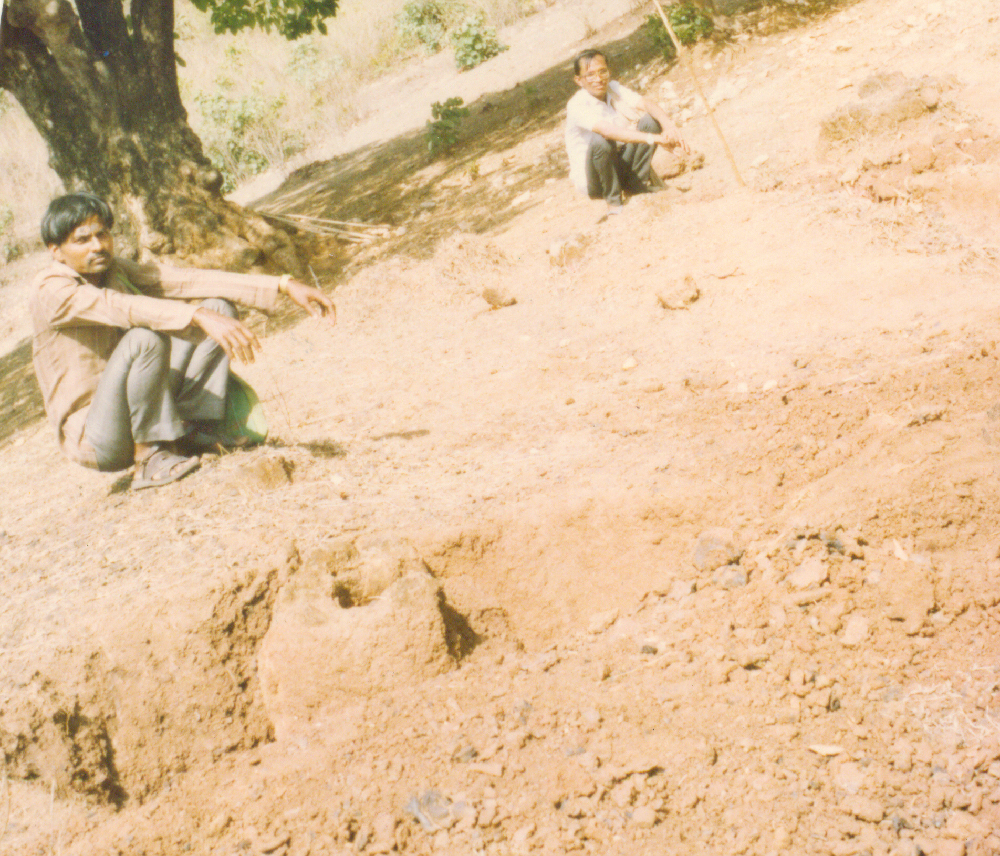
\includegraphics[scale=1.8]{images/chapter-7/fig052A.jpg}
\caption{A deserted site Bishunpur, Jharkhand}\label{chapter-7-fig52A}
\end{figure}
\begin{figure}[H]
\renewcommand{\thefigure}{52B}
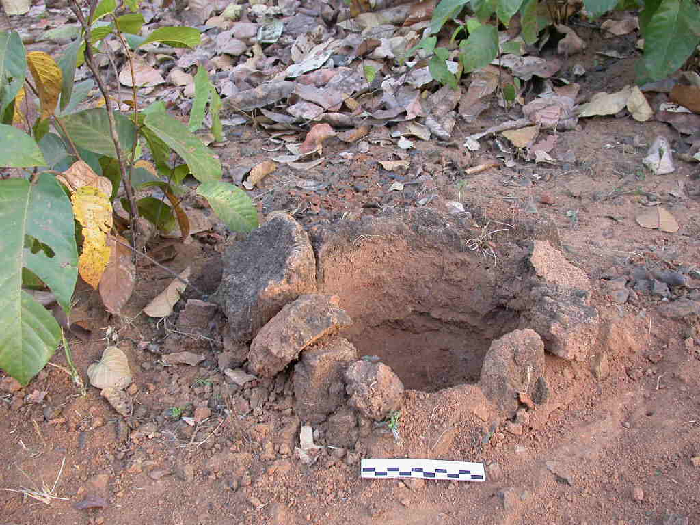
\includegraphics[scale=1.4]{images/chapter-7/fig052B.jpg}
\caption{Pipra}\label{chapter-7-fig52B}
\end{figure}

\newpage

\begin{figure}[H]
\renewcommand{\thefigure}{52C}
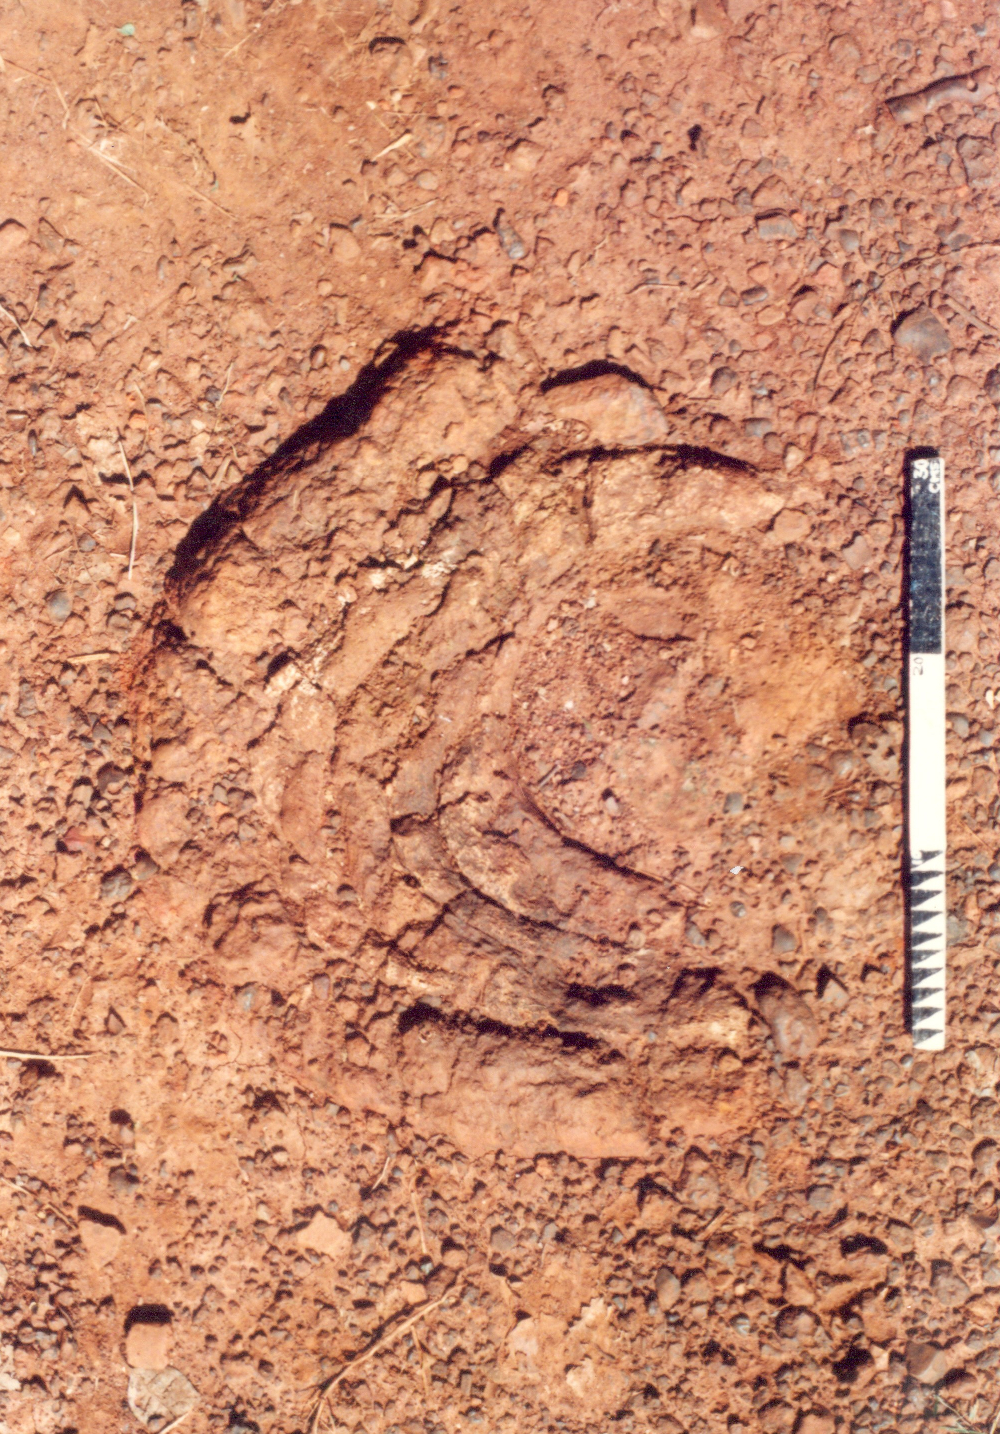
\includegraphics[scale=1.2]{images/chapter-7/fig052C.jpg}
\caption{Broken furnace, Odisha}\label{chapter-7-fig52C}
\end{figure}
\begin{figure}[H]
\renewcommand{\thefigure}{53A}
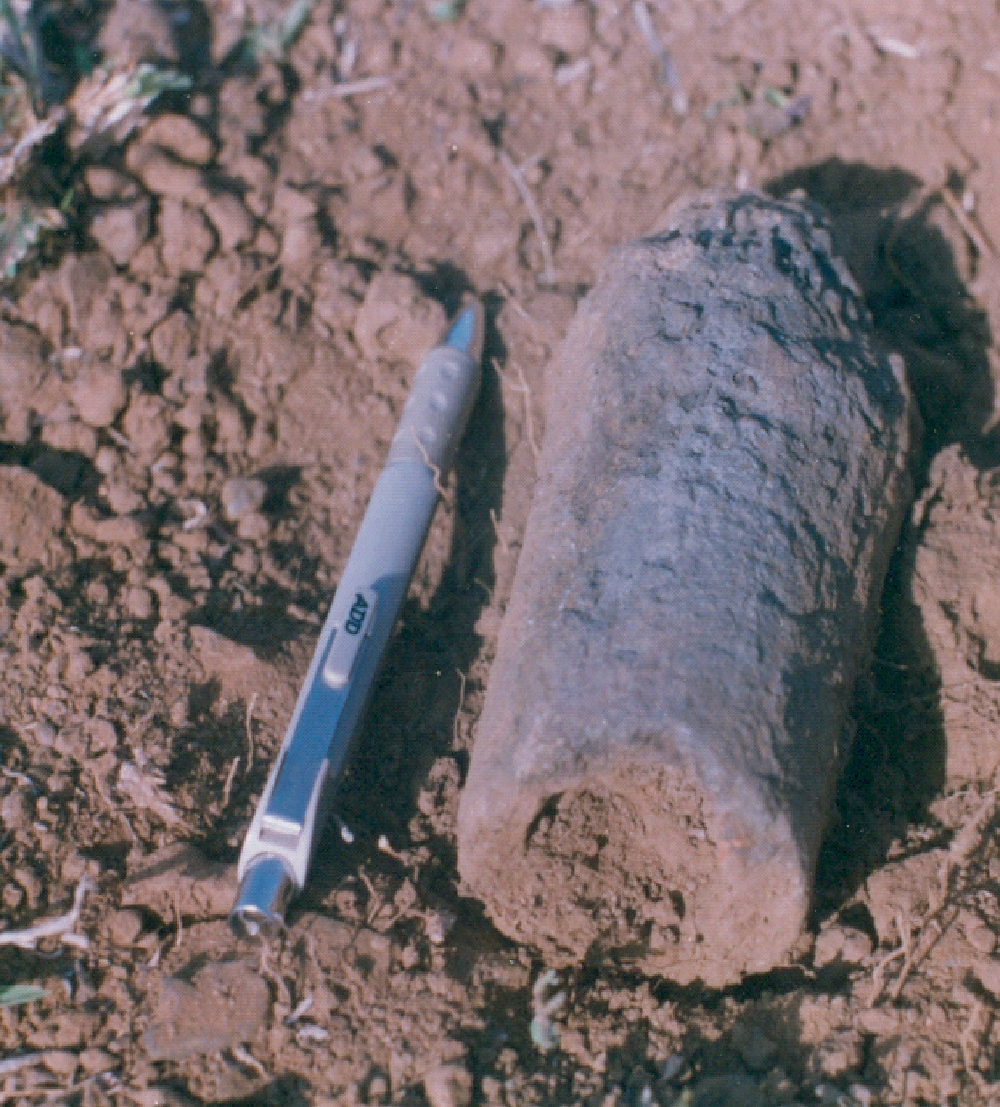
\includegraphics[scale=1.5]{images/chapter-7/fig053A.jpg}
\caption{Abandoned sites of traditional iron working, Sonbhadra}\label{chapter-7-fig53A}
\end{figure}

\newpage

\begin{figure}[H]
\renewcommand{\thefigure}{53B}
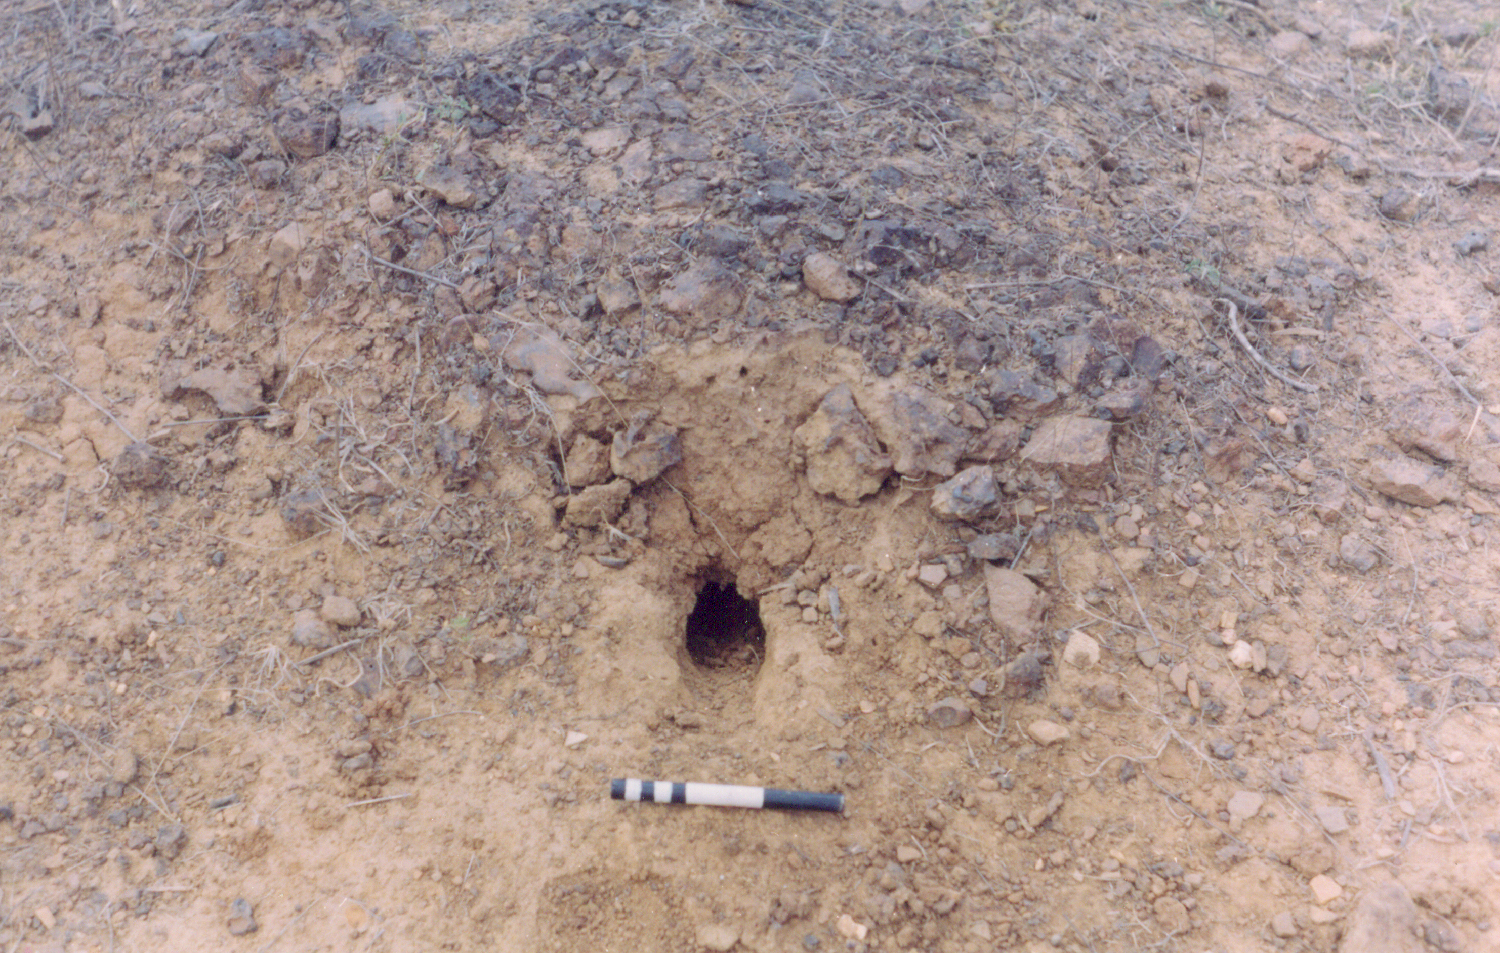
\includegraphics[scale=1.5]{images/chapter-7/fig053B.jpg}
\caption{Abandoned sites of traditional iron working, Sonbhadra}\label{chapter-7-fig53B}
\end{figure}
\begin{figure}[H]
\renewcommand{\thefigure}{53C}
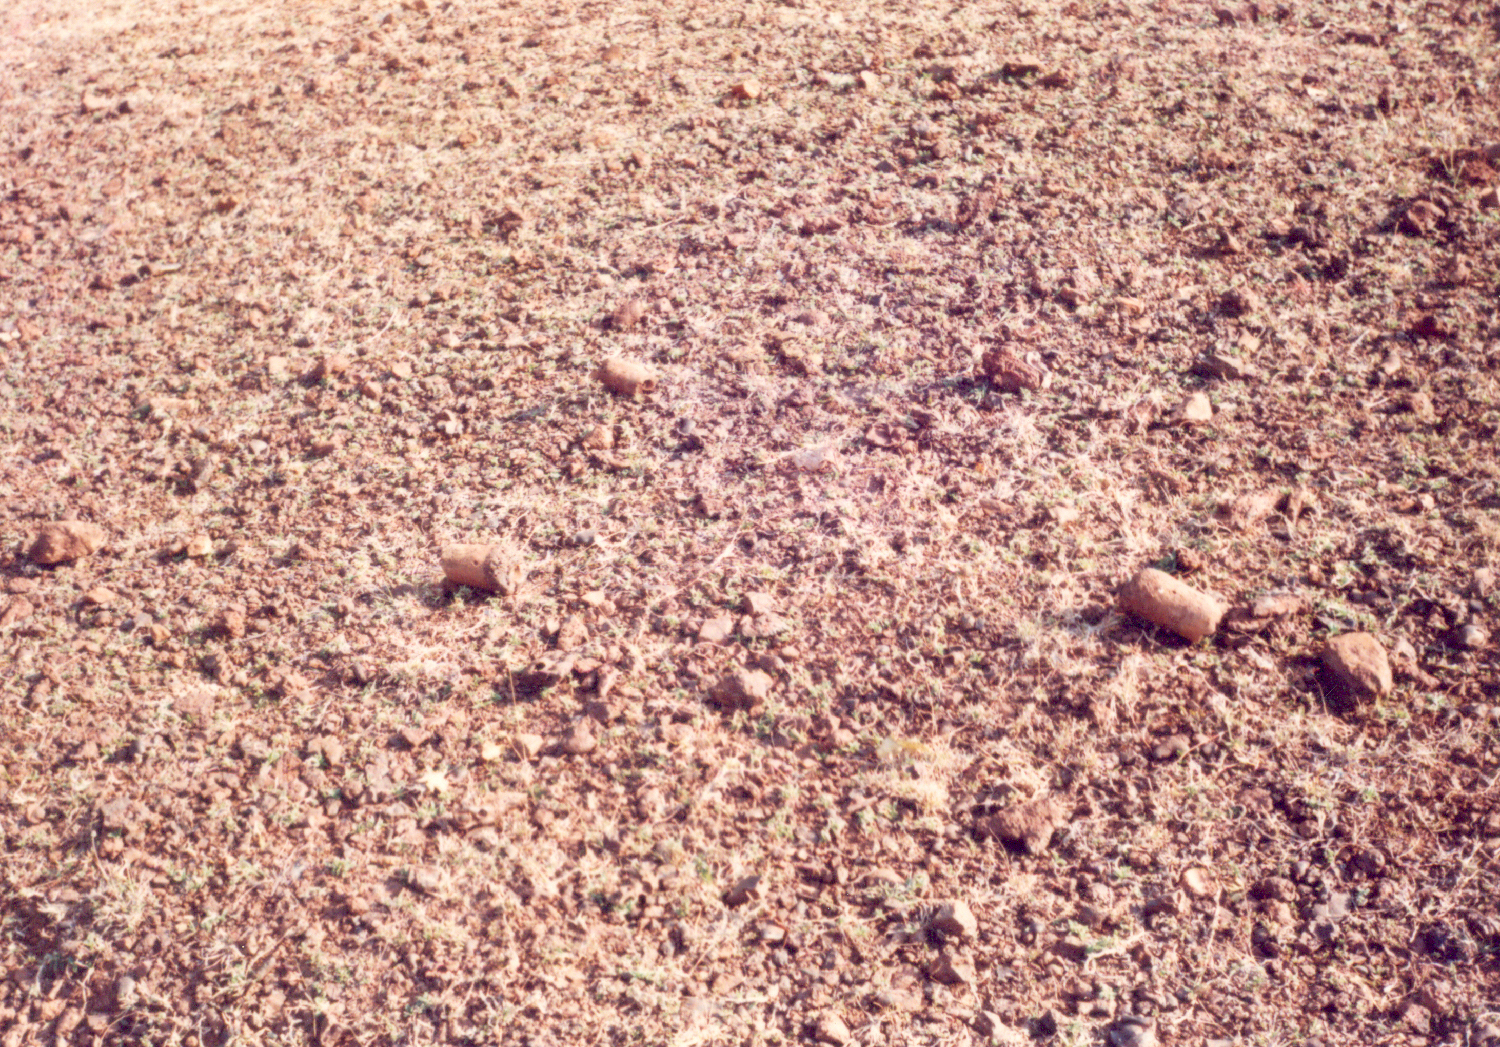
\includegraphics[scale=1.5]{images/chapter-7/fig053C.jpg}
\caption{Sonbhadra}\label{chapter-7-fig53C}
\end{figure}

\newpage

\begin{figure}[H]
\renewcommand{\thefigure}{53D}
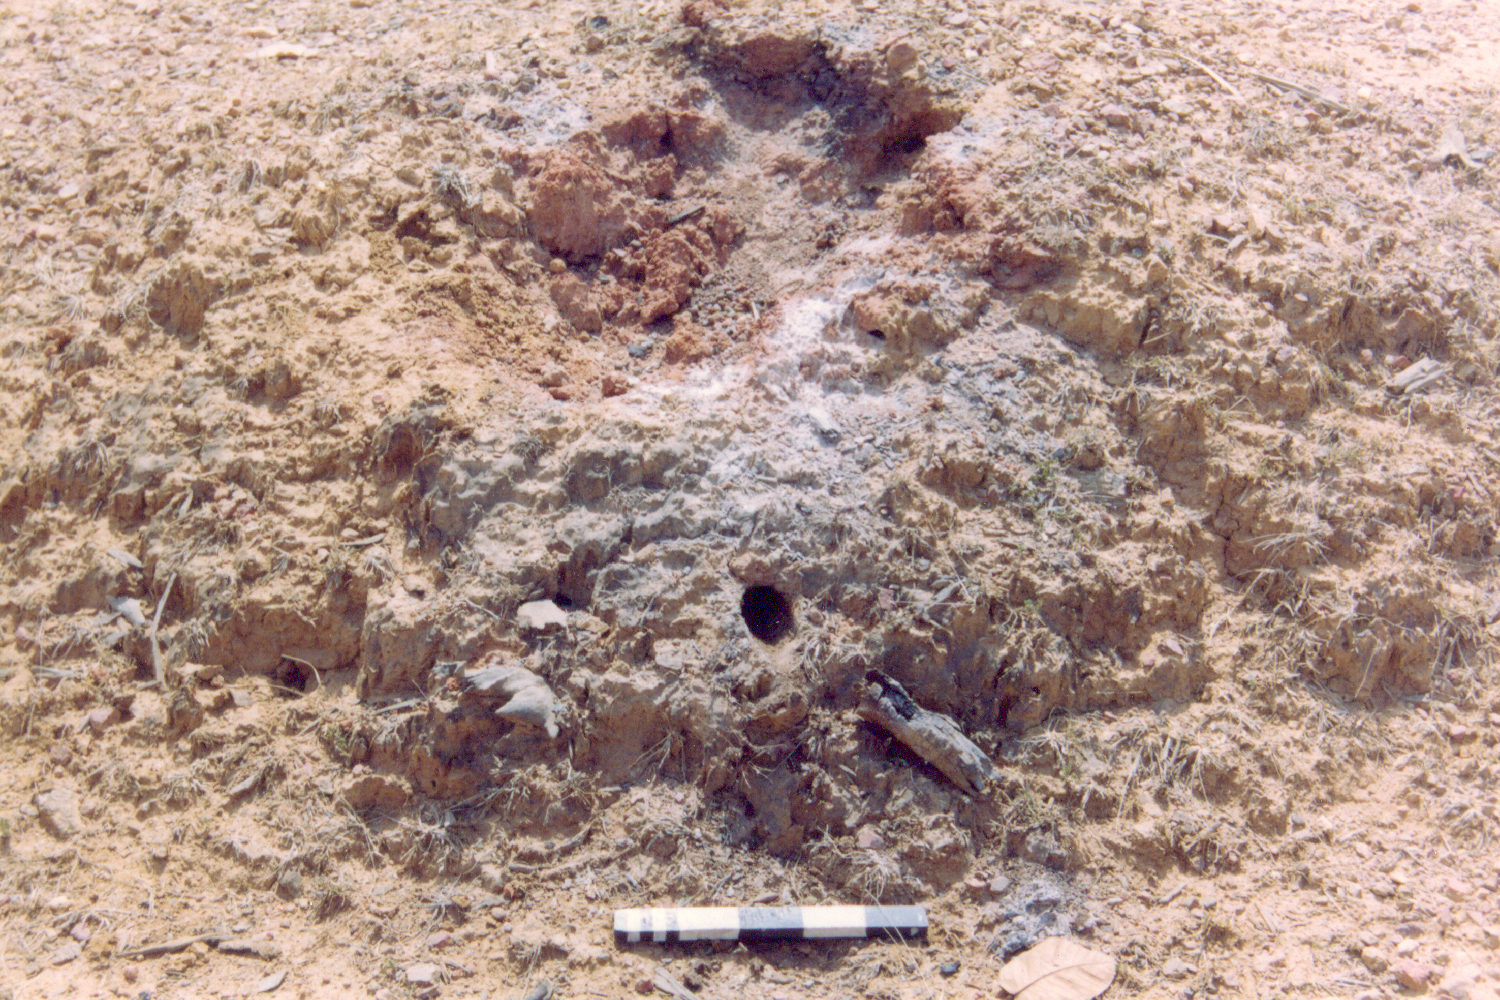
\includegraphics[scale=1.5]{images/chapter-7/fig053D.jpg}
\caption{Iron smelting site Sonbhadra}\label{chapter-7-fig53D}
\end{figure}
\begin{figure}[H]
\renewcommand{\thefigure}{53E}
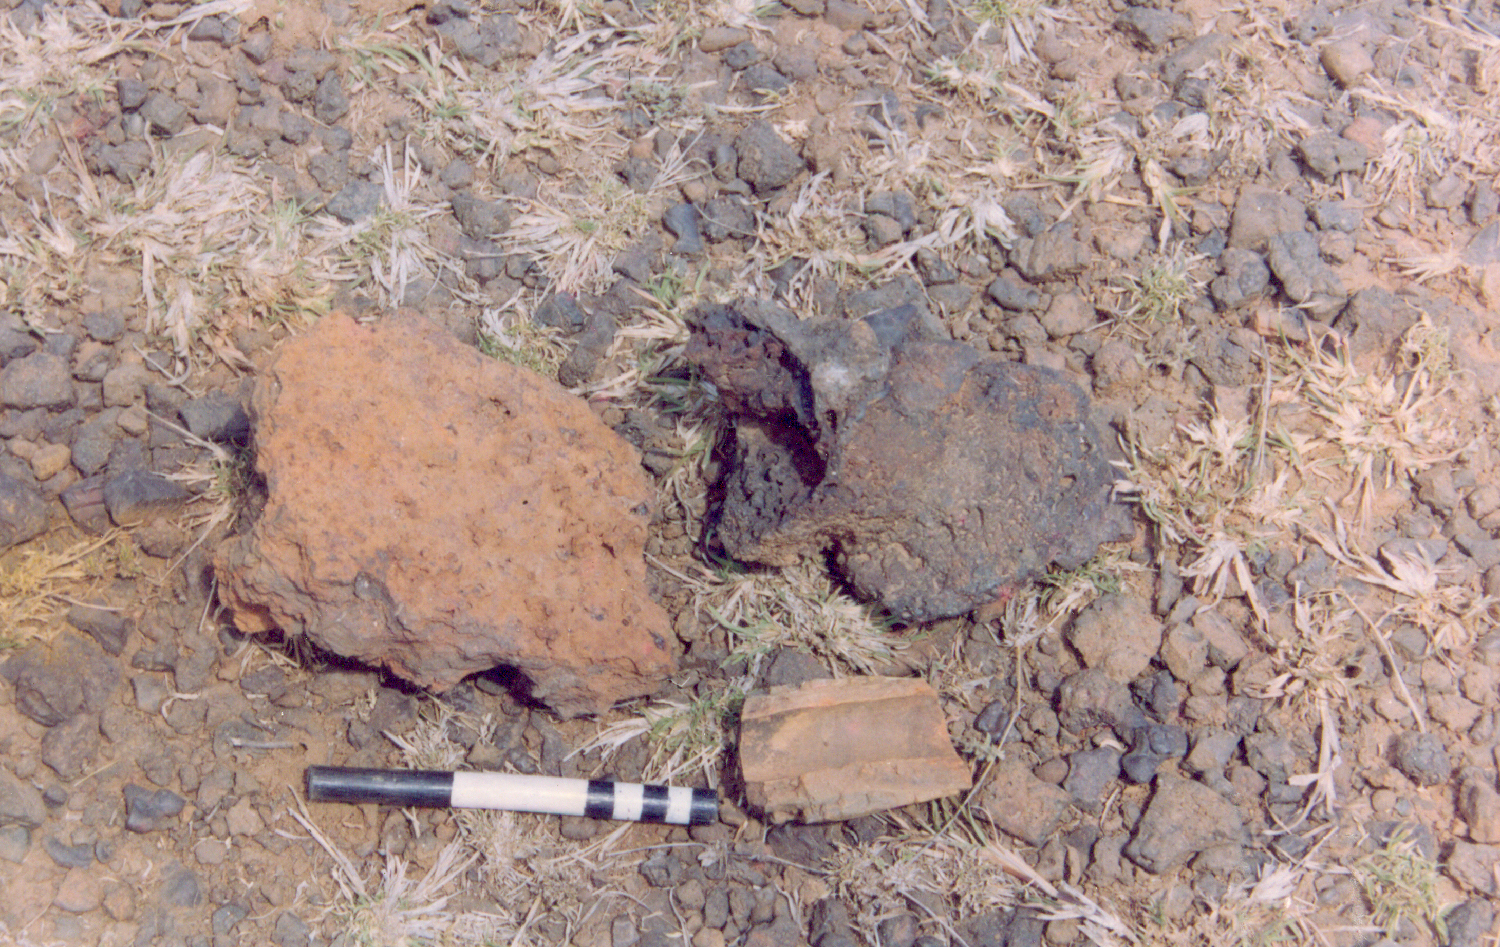
\includegraphics[scale=1.5]{images/chapter-7/fig053E.jpg}
\caption{Iron slag Lump}\label{chapter-7-fig53E}
\end{figure}

\newpage

\begin{figure}[H]
\setcounter{figure}{53}
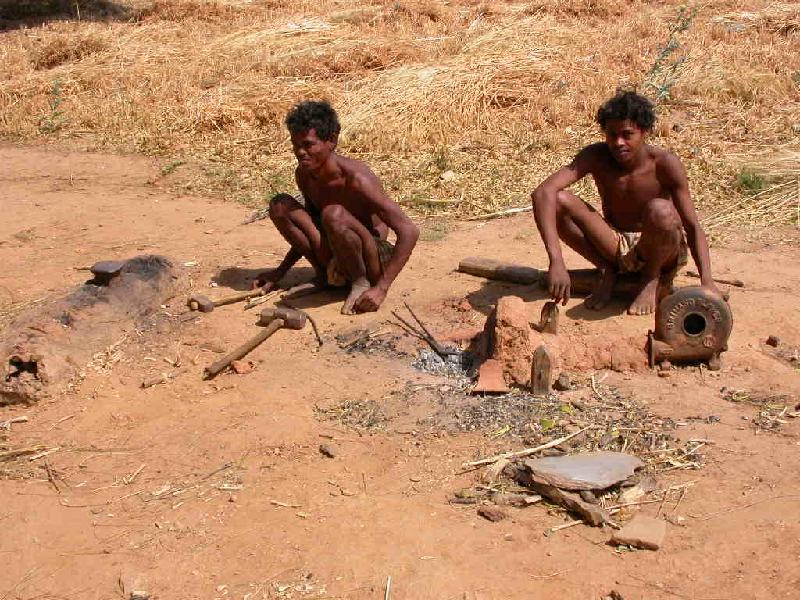
\includegraphics[scale=1.4]{images/chapter-7/fig054.jpg}
\caption{A Sidhi MP}\label{chapter-7-fig54}
\end{figure}
\begin{figure}[H]
\renewcommand{\thefigure}{55A}
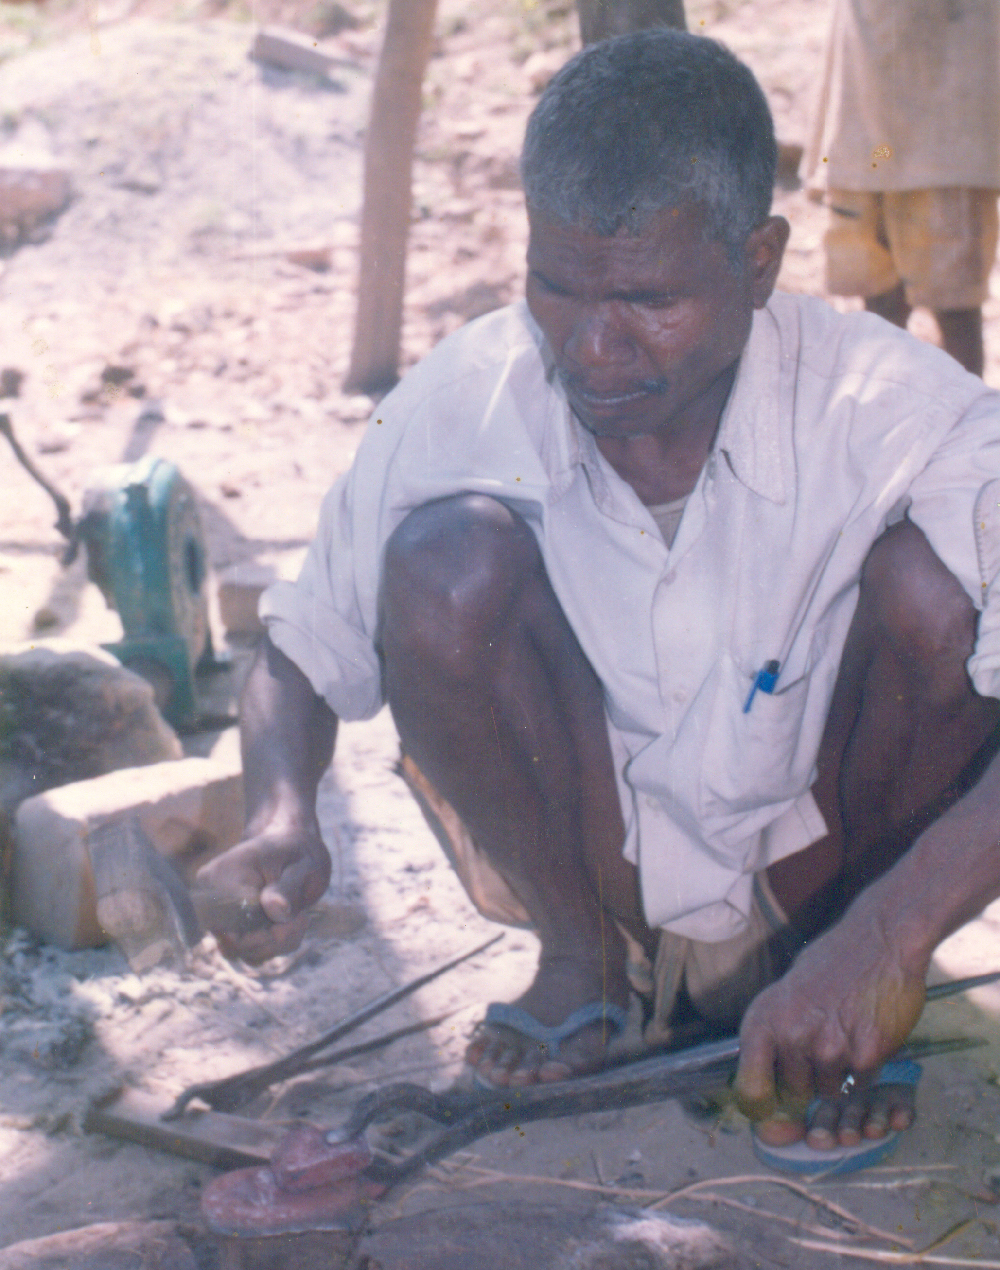
\includegraphics[scale=1.35]{images/chapter-7/fig055A.jpg}
\caption{Sonbhadra}\label{chapter-7-fig55A}
\end{figure}

\newpage

\begin{figure}[H]
\renewcommand{\thefigure}{55B}
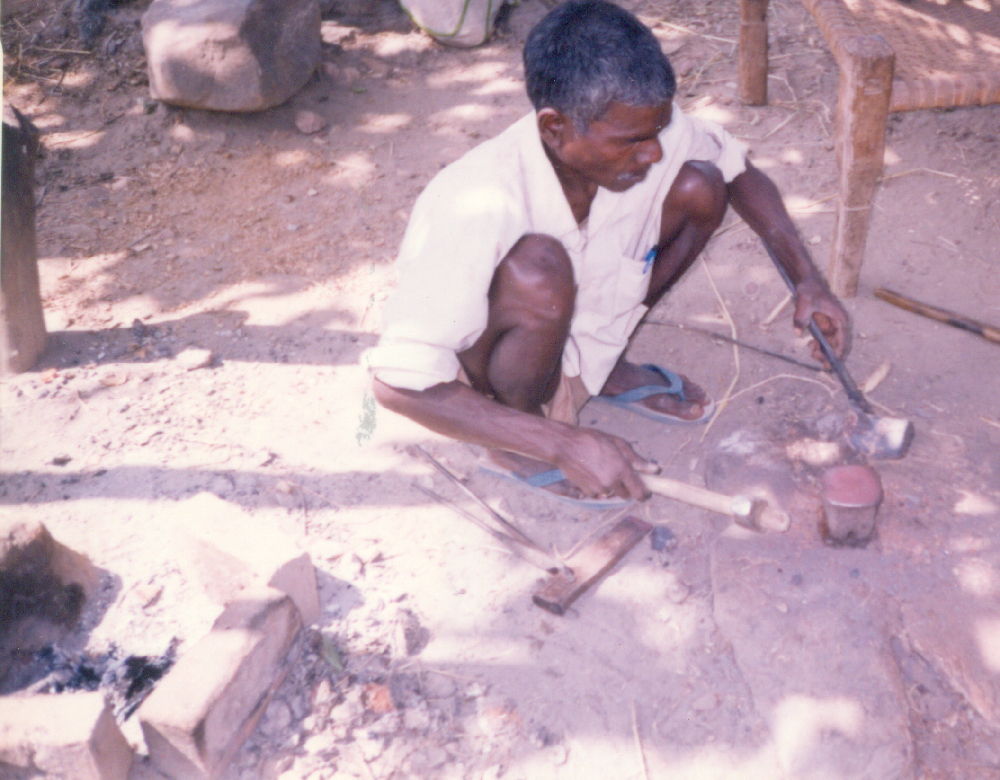
\includegraphics[scale=1.7]{images/chapter-7/fig055B.jpg}
\caption{Sonbhadra}\label{chapter-7-fig55B}
\end{figure}
\begin{figure}[H]
\setcounter{figure}{55}
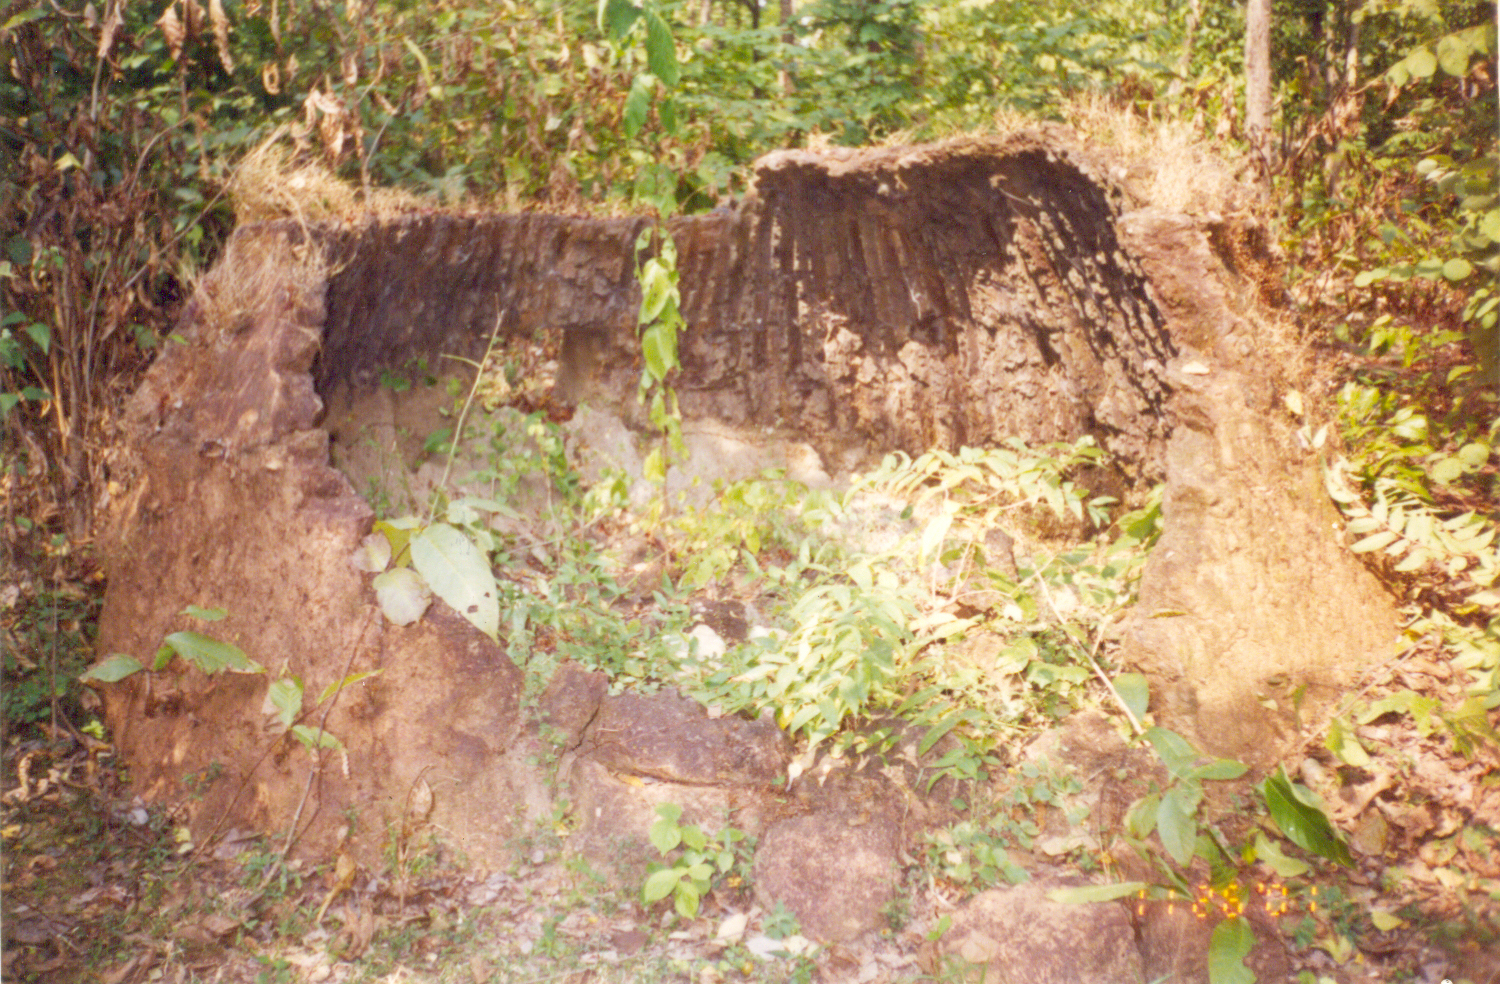
\includegraphics[scale=1.5]{images/chapter-7/fig056.jpg}
\caption{Coal Making Kilns, Singhbhum, Jharkhand}\label{chapter-7-fig56}
\end{figure}

\newpage

\begin{figure}[H]
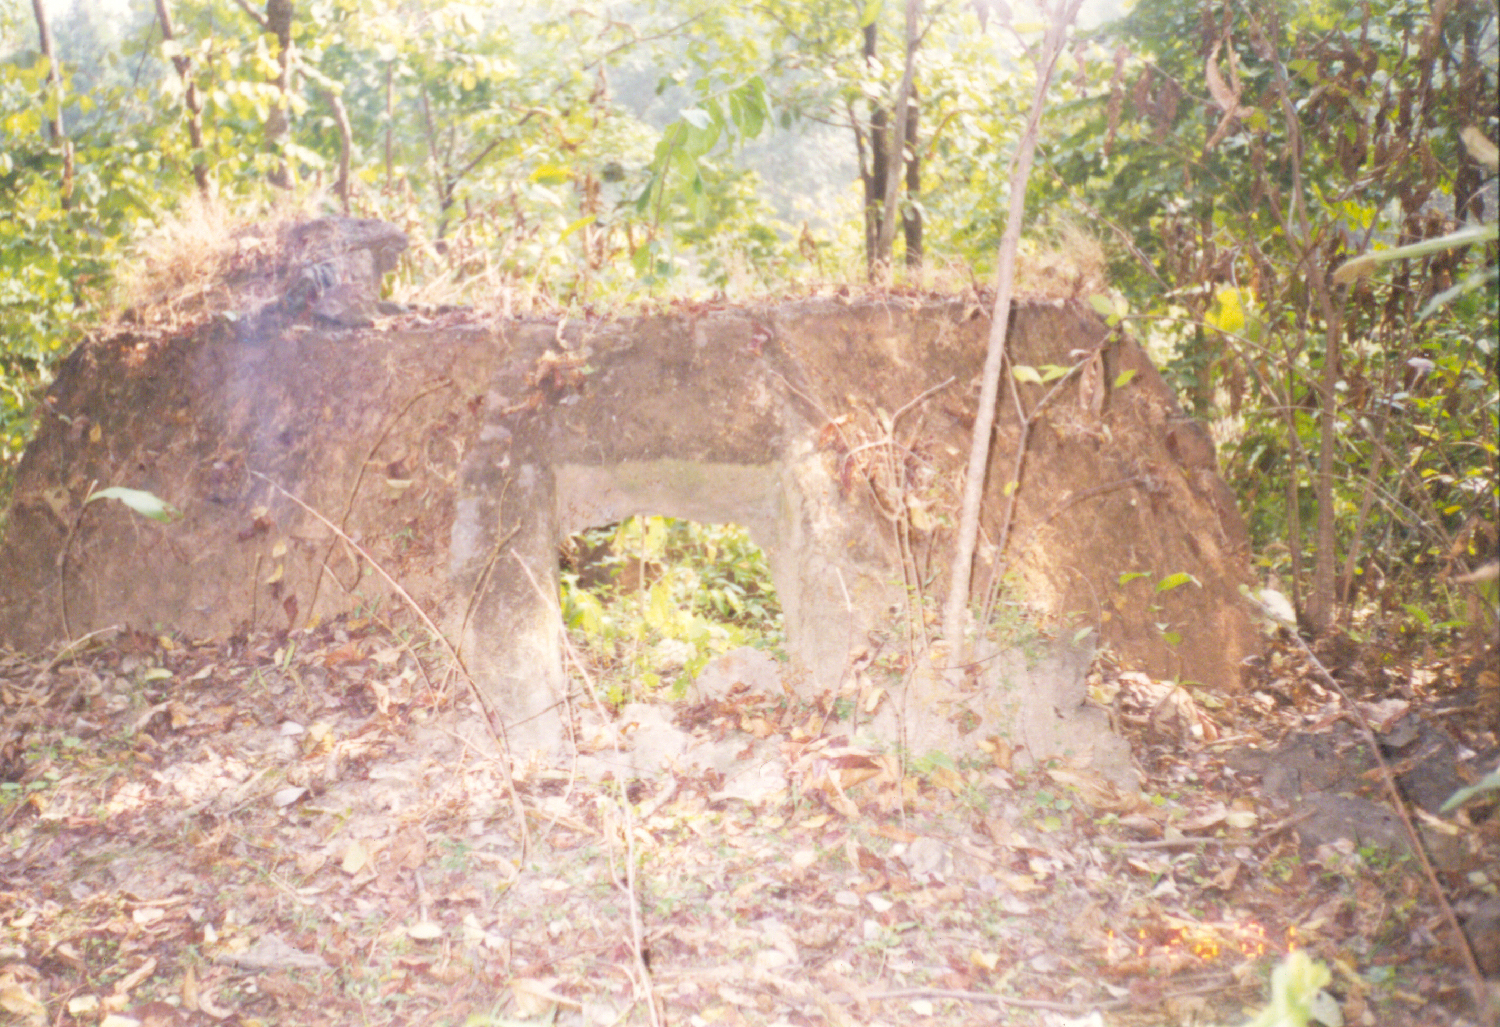
\includegraphics[scale=1.5]{images/chapter-7/fig057.jpg}
\caption{Coal making kilns, Singhbhum, Jharkhand}\label{chapter-7-fig57}
\end{figure}
\begin{figure}[H]
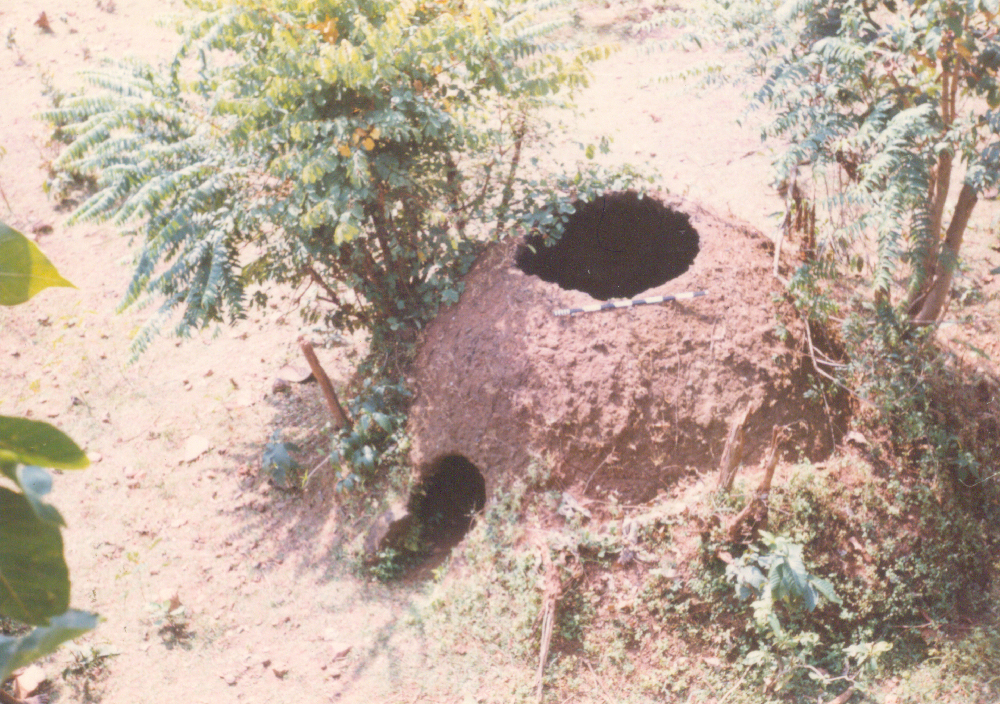
\includegraphics[scale=2.3]{images/chapter-7/fig058.jpg}
\caption{Charcoal making kiln, Odisha}\label{chapter-7-fig58}
\end{figure}

\newpage

\begin{figure}[H]
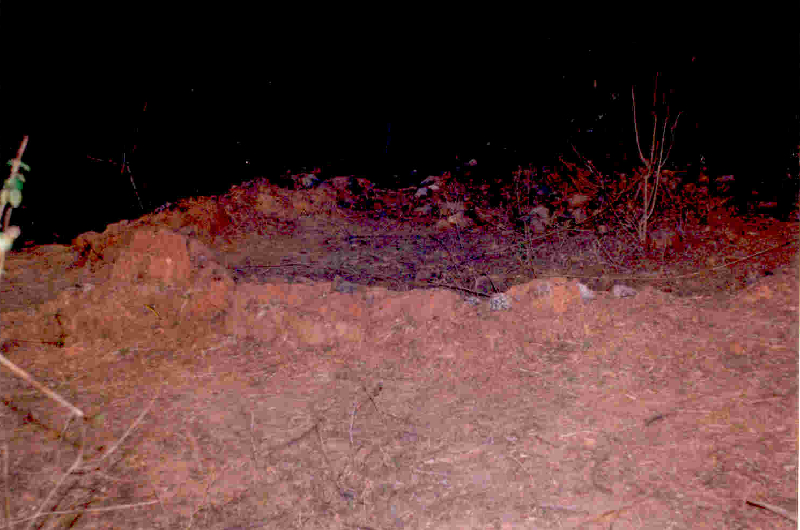
\includegraphics[scale=1.4]{images/chapter-7/fig059.jpg}
\caption{Traces of charcoal making kiln, Sonbhadra}\label{chapter-7-fig59}
\end{figure}

It may not be pragmatic to talk of revival of the tradition at the cost of modern industries but the two may be allowed to co-exist. In the modern times of environmental degradation and overuse of non-renewable resources, growing trees will go a long way. Tree plantation is a great option and this does not need elaboration. We may do this for the benefit of a variety of industries including the traditional iron working. This will have a long time effect on economic, social and cultural ecology of the country, especially when the world is talking about `small is beautiful'. While the traditional iron industry will support a section of sizable population of traditional ironworkers and help revive a traditional industry, it will also help them lead a life with self-respect. This will eventually help preserve our technological heritage and a legacy of the past.

\vspace{-.3cm}

\theendnotes

\label{endchapter7}


%~ \noindent \textbf{\large Notes:}

%~ ${}^1$Leuva has referred to the episode of Virochan, the Great Asur in Chhandogya Upanishad who misinterpreted the teachings of Prajapati about Atman and advised his fellowmen to bury their dead, ( Leuva in the preface, xiii)

%~ ${}^2$The excavation of Khairdih in district Ballia U.P. has yielded small handled pestle and a footed longish quern from a workshop area (Fig. \ref{10 A,B}). Similarly from Latif Shah several such crushing stones- pestles and querns have been discovered from iron working workshops and smithies (Fig. \ref{10C})

%~ ${}^3$Experiments carried out by Prakash and the author with Waddraffnagar Agrarias have shown that even poor grade charcoal could be used in these furnaces but for this the smelters have to be trained and prepared mentally to change the air blowing rate.

